% for two sided printing
%\documentclass[11pt,a4paper,twoside]{book}
% for one sided printing
\documentclass[11pt,a4paper,oneside]{book}
% A few packages that you might need - I have included all the ones that are needed for this template to work correctly, plus a few more. If you wish to do more with Latex then you may need to import other ones. 
\usepackage{amsmath,amssymb,amsthm,color,enumerate,graphicx,stackrel,natbib,setspace,ifthen,url,array,theorem,pifont}
\usepackage{lscape}
\usepackage{placeins}
\usepackage{multirow}
\usepackage{fancyhdr}
\usepackage{emptypage}
% For printing with binding
\usepackage[inner=4cm,outer=2cm,top=2.5cm,bottom=3cm]{geometry}
% For pdf or printing without binding
% \usepackage[inner=3cm,outer=3cm,top=2.5cm,bottom=3cm]{geometry}
\usepackage[sc]{titlesec}

%\usepackage[toc,page]{appendix}
\usepackage[titletoc,title]{appendix}
%\input{FloatSettings} % For things like figures and tables
%\input{BibSettings}   % For bibliographies
\linespread{1.3}
% Title Settings
\setcounter{secnumdepth}{3}
\setcounter{tocdepth}{3}
\usepackage{hyperref}
\usepackage{doi}

% For subfigures
\usepackage{subcaption}
\captionsetup{compatibility=false}

% For turning " into ``
\usepackage [english]{babel}
\usepackage [autostyle, english = american]{csquotes}
\MakeOuterQuote{"}

% No indentation for new paragraphs
\usepackage[parfill]{parskip}
\setlength\parindent{0pt}


% For tables
\usepackage{tabularx}
\usepackage{booktabs}

% Fix weird whitespace formatting for URLs in bibliography
\usepackage{xurl}

% \documentclass{scrreprt}
\makeatletter
\usepackage{color}
\definecolor{lightgray}{rgb}{0.95, 0.95, 0.95}
\definecolor{darkgray}{rgb}{0.4, 0.4, 0.4}
%\definecolor{purple}{rgb}{0.65, 0.12, 0.82}
\definecolor{editorGray}{rgb}{0.95, 0.95, 0.95}
\definecolor{editorOcher}{rgb}{1, 0.5, 0} % #FF7F00 -> rgb(239, 169, 0)
\definecolor{editorGreen}{rgb}{0, 0.5, 0} % #007C00 -> rgb(0, 124, 0)
\definecolor{orange}{rgb}{1,0.45,0.13}		
\definecolor{olive}{rgb}{0.17,0.59,0.20}
\definecolor{brown}{rgb}{0.69,0.31,0.31}
\definecolor{purple}{rgb}{0.38,0.18,0.81}
\definecolor{lightblue}{rgb}{0.1,0.57,0.7}
\definecolor{lightred}{rgb}{1,0.4,0.5}
\usepackage{upquote}
\usepackage{listings}
% CSS
\lstdefinelanguage{CSS}{
  keywords={color,background-image:,margin,padding,font,weight,display,position,top,left,right,bottom,list,style,border,size,white,space,min,width, transition:, transform:, transition-property, transition-duration, transition-timing-function},	
  sensitive=true,
  morecomment=[l]{//},
  morecomment=[s]{/*}{*/},
  morestring=[b]',
  morestring=[b]",
  alsoletter={:},
  alsodigit={-}
}

% JavaScript
\lstdefinelanguage{JavaScript}{
  morekeywords={typeof, new, true, false, catch, function, return, null, catch, switch, var, if, in, while, do, else, case, break},
  morecomment=[s]{/*}{*/},
  morecomment=[l]//,
  morestring=[b]",
  morestring=[b]'
}

\lstdefinelanguage{HTML5}{
  language=html,
  sensitive=true,	
  alsoletter={<>=-},	
  morecomment=[s]{<!-}{-->},
  tag=[s],
  otherkeywords={
  % General
  >,
  % Standard tags
	<!DOCTYPE,
  </html, <html, <head, <title, </title, <style, </style, <link, </head, <meta, />,
	% body
	</body, <body,
	% Divs
	</div, <div, </div>, 
	% Paragraphs
	</p, <p, </p>,
	% scripts
	</script, <script,
  % More tags...
  <canvas, /canvas>, <svg, <rect, <animateTransform, </rect>, </svg>, <video, <source, <iframe, </iframe>, </video>, <image, </image>, <header, </header, <article, </article
  },
  ndkeywords={
  % General
  =,
  % HTML attributes
  charset=, src=, id=, width=, height=, style=, type=, rel=, href=,
  % SVG attributes
  fill=, attributeName=, begin=, dur=, from=, to=, poster=, controls=, x=, y=, repeatCount=, xlink:href=,
  % properties
  margin:, padding:, background-image:, border:, top:, left:, position:, width:, height:, margin-top:, margin-bottom:, font-size:, line-height:,
	% CSS3 properties
  transform:, -moz-transform:, -webkit-transform:,
  animation:, -webkit-animation:,
  transition:,  transition-duration:, transition-property:, transition-timing-function:,
  }
}

% For Typescript code listings
\lstdefinestyle{htmlcssjs} {%
  % General design
%  backgroundcolor=\color{editorGray},
  basicstyle={\footnotesize\ttfamily},   
  frame=b,
  % line-numbers
  xleftmargin={0.75cm},
  numbers=left,
  stepnumber=1,
  firstnumber=1,
  numberfirstline=true,	
  % Code design
  identifierstyle=\color{black},
  keywordstyle=\color{blue}\bfseries,
  ndkeywordstyle=\color{editorGreen}\bfseries,
  stringstyle=\color{editorOcher}\ttfamily,
  commentstyle=\color{brown}\ttfamily,
  % Code
  language=HTML5,
  alsolanguage=JavaScript,
  alsodigit={.:;},	
  tabsize=2,
  showtabs=false,
  showspaces=false,
  showstringspaces=false,
  extendedchars=true,
  breaklines=true,
  % German umlauts
  literate=%
  {Ö}{{\"O}}1
  {Ä}{{\"A}}1
  {Ü}{{\"U}}1
  {ß}{{\ss}}1
  {ü}{{\"u}}1
  {ä}{{\"a}}1
  {ö}{{\"o}}1
}


\begin{document}
\pagestyle{plain}
\frontmatter
%Create a title page
\begin{titlepage} % Suppresses displaying the page number on the title page and the subsequent page counts as page 1
	\newcommand{\HRule}{\rule{\linewidth}{0.5mm}} % Defines a new command for horizontal lines, change thickness here
	
	\center % Centre everything on the page
	%------------------------------------------------
	%	Headings
	%------------------------------------------------	
	\textsc{\LARGE University College London}\\[1.5cm] % Main heading institution
	
	\textsc{\Large Department of Computer Science}\\[0.5cm] % Major heading department
	
	\textsc{\large A thesis submitted in partial fulfilment of the requirements for the degree of Master of Science in Financial Technology, University College London}\\[0.5cm] % Minor heading such as course title	
	%------------------------------------------------
	%	Title
	%------------------------------------------------
	\HRule\\[0.4cm]
	\textsc{\huge Streamlining Derivative Trading: Enhanced Liquidity and Risk Mitigation with Blockchain-based Tokenised Collateral Management }\\[0.4cm] % Title of your document
	\HRule\\[1.5cm]
	%------------------------------------------------
	%	Author and Supervisor
	%------------------------------------------------
	{\large\textit{Author}}\\
	Vincenzo \textsc{Incutti} % Your name
	\vfill
	\begin{minipage}{0.48\textwidth}
		\begin{flushleft}
			\large
			\textit{Academic Supervisor}\\
			Prof. Christopher D. \textsc{Clack}\\ % Supervisor's name
			\textsc{Department of Computer Science}\\
			\textsc{University College London}
		\end{flushleft}
	\end{minipage}
	~% Fill in the next one for your industrial supervisor - if you do not have one put your second marker
	\begin{minipage}{0.48\textwidth}
            \begin{flushright}
                \large
                \textit{Industrial Supervisors}\\
                \makebox[0.4\textwidth][r]{Richard \textsc{Barker (CEO)},} \\
                \makebox[0.4\textwidth][r]{Gerard \textsc{Banaszkiewicz (COO)},} \\
                \makebox[0.4\textwidth][r]{Steve \textsc{Haigh (CTO)},} \\
                \makebox[0.4\textwidth][r]{John \textsc{Anderson (CPO)},} \\
                \makebox[0.4\textwidth][r]{Nazish \textsc{Zaidi (Lead Business Analyst)},} \\
                \makebox[0.4\textwidth][r]{Stephen \textsc{Ashworth (Head of Platform)},} \\
                \makebox[0.4\textwidth][r]{Brendan \textsc{Bradely (Chairman)},} \\
                \textsc{Tokenovate} \\ %Company name
        \end{flushright}
    \end{minipage}
	%------------------------------------------------
	%	Date
	%------------------------------------------------	
	\vfill\vfill\vfill % Position the date 3/4 down the remaining page	
	
	{\large\textit\today} % Date, change the \today to a set date if you want to be precise
	
	%------------------------------------------------
	%	Logo
	%------------------------------------------------
       
\includegraphics[width=0.2\textwidth]{ucl_logo}\\[1cm] % Include a department/university logo - this will require the graphicx package
	%------------------------------------------------
	%	Disclaimer
	%------------------------------------------------
	
	% Uncomment one of the following statements as appropriate.
	
	 This dissertation is submitted as part requirement for the MSc Financial Technology degree at UCL. It is substantially the result of my own work except where explicitly 	indicated in the text. The report may be freely copied and distributed provided the source is explicitly acknowledged.
	 
	 %The dissertation may be freely copied and distributed provided the source is explicitly acknowledged.

	%Or if your project includes information that prevents it from being more widely circulated:
	
	% This dissertation is submitted as part requirement for the MSc ? degree at UCL. It is substantially the result of my own work except where explicitly 	indicated in the text. The dissertation will be distributed to the internal and external examiners, but thereafter may not be copied or distributed except 	with permission from the author.

	%\vfill % Push the date up 1/4 of the remaining page
	
\end{titlepage}
\clearpage 
\newpage 


\section*{Abstract}
The aim of this study is to address the operational inefficiencies plaguing the collateral management systems in financial derivative trading, which have far-reaching implications for market liquidity and efficiency. To this end, we introduce a blockchain-based solution that automates settlement and reconciliation processes, traditionally managed by intermediary clearing houses. Our methodology involves the creation of a tokenised collateral system on the Bitcoin Satoshi Vision (BSV) blockchain, adhering to industry standards set by the International Swaps and Derivative Association (ISDA) and utilizing sCrypt, a Typescript-based Domain Specific Language to write smart contracts. A proof of concept tokenising crude oil as collateral is also presented. Our research reveals that while the BSV ecosystem is still in its infancy, greater collaboration between financial and tech sectors is essential for a seamless transition to a blockchain-based financial infrastructure. The study also sheds light on the technical hurdles in adapting existing ISDA frameworks to blockchain technology.
\newpage 
\section*{Acknowledgments}
I wish to express my gratitude to my supervisor, Dr. Christopher D. Clack, for his invaluable assistance throughout the drafting of this dissertation. Additionally, I extend my appreciation to the entire team at Tokenovate Ltd, with a special mention of John, Nazish, and Stephen, for their invaluable business insights and guidance on the practical applications of this work. I would also like to acknowledge the postgraduate students who are working on their own dissertations under Dr. Clack's supervision, especially Finn, for being a source of inspiration and providing valuable feedback on my work. Finally, my heartfelt thanks go to my flatmate, Lukas, for the unwavering moral support during the challenging months of research and writing.

\newpage
% The table of contents, list of figures and list of tables go here
\setcounter{tocdepth}{3} 
% Setting this higher means you get contents entries for
%  more minor section headers.
\cleardoublepage
\tableofcontents
\cleardoublepage
\listoffigures
\cleardoublepage
\listoftables

% Start the main part of the document here.

% ################ CHAPTER 1 ################ 
\mainmatter
\chapter{Introduction}
\label{ch:Introduction}
Derivatives \citep{quail2002financial}, as intricate financial instruments, rely on a myriad of interconnected systems—spanning finance, economics, law, and technology—for effective trading. The complex interplay between these systems often leads to conflicts that necessitate legal resolution or the cessation of trades to reconcile discrepancies in counterparties' information.

The 2008 financial crisis prompted international bodies to enforce stricter regulations to mitigate systemic risk \citep{ferran2012regulatory}. However, these expanded regulatory and legislative measures were imposed on an antiquated technological infrastructure not originally designed to accommodate them.

A challenging aspect of derivative trading is the management and payment of collateral. Collateral, assets temporarily transferred between parties, acts as a safeguard against counterparty risk during the derivative lifecycle. The current collateral administration process is fraught with issues. Movement of collateral assets often incurs considerable costs and operational overheads, sometimes necessitating the physical transfer of assets to third-party accounts. According to a report by the European Commission, the European Securities and Markets Authority (ESMA) has identified more than 400 trading data contributors, each currently reporting data in different manners \citep{eu_data_fragmentation}. The reason behind this is that current reporting
standards leave discretion in the interpretation of various reporting data fields, creating low quality market data reports and resulting in regulatory reporting
arbitrage, sometimes even paving the ground for deliberate mis-reporting of trades (the Financial Conduct Authority (FCA) constantly updates their list of reporting transaction fines \citep{fca_reporting_fines}, from whose frequency and magnitude we can infer the gravity of the issue). These inefficiencies frequently compel third parties to hold positions overnight and bridge unexpected holdings.

The International Swaps and Derivatives Association (ISDA) \citep{isda_home} has been working to standardize, digitize, and automate several crucial processes of derivative trading. A key focus has been the utilization of Smart Derivative Contracts to enhance infrastructure and mitigate challenges. By leveraging the transparency, accountability, and decentralization inherent in blockchain technology, Smart Derivative Contracts could automate many operational clauses of derivative agreements \citep{clack2018temporal}. This automation could reduce manual input (and thus error), cut reconciliation costs, improve regulatory reporting, and streamline the collateral allocation process. The end results could be diminished balance sheet risk and enhanced capital allocation for liquidity creation.

This dissertation proposes a tokenized collateral system implemented via smart contracts on the Bitcoin Satoshi Vision (BSV) blockchain \citep{bsv_home}. The aim is to refine the derivative trading lifecycle while adhering to existing regulatory, legislative, and business standards and processes. It evaluates the advantages of using the BSV blockchain to represent collateral, explores potential future directions for a settlement and payment layer trading such collateral, and analyzes the legal, financial, and economic implications of tokenized collateral. It also compares BSV with more widely-adopted distributed ledger systems like Ethereum \citep{dannen2017introducing} and Bitcoin \citep{nakamoto2008bitcoin}.

The research maps the collateral representation from the ISDA Common Domain Model (CDM) \citep{isda_cdm_factsheet} — the industry's most widely accepted standard—to one in sCrypt \citep{scrypt_home}, a domain-specific language (DSL) based on TypeScript \citep{typescript_home} for writing smart contracts on BSV. It examines the fractionalization of collateral value via satoshis and explores the use of off-chain oracles for providing real-world data streams to smart contracts.
\section{Objectives and Contributions of the Thesis}
\label{sec:objectives}

The innovative contributions of this dissertation exist within the intersection of blockchain technology and the traditionally structured realm of collateral management for derivative trading. This work illuminates the potential for this technology to streamline, secure, and transform the intricate processes involved in managing collateral.

Firstly, a substantial contribution of this work involves developing a concrete methodology for tokenising underlying collateral assets. Tokenisation, as examined in this dissertation, is a procedure that embodies the translation of the economic and legal rights associated with a real-world asset into a digital token. This mechanism makes the asset easily transferable and divisible, enabling more efficient management and real-time valuations. In essence, the endeavour to precisely define the method and expected value outcomes of tokenisation provides a gateway to greater liquidity, improved accessibility, and the potential for enhanced market depth and breadth.

Secondly, this work outlines a robust representation for these tokenised assets in the digital space, which is often referred to as a "digital twin". Specifically, this involves demonstrating in code how these digital representations can encapsulate their unique value per asset type. This novel contribution paves the way for an improved system of representing physical assets digitally. It enhances the overall understanding and representation of the asset and, in the process, facilitates more accurate and efficient asset management.

The creation of a Proof of Concept (PoC) forms the third innovative contribution. The PoC, demonstrated in code form, goes beyond the theoretical assertions to offer a hands-on, tangible representation of the proposed solution. It provides a compelling representation of how such a system might operate in practice, adding credibility to the proposed methods.

In addition, the benefits of the proposed solution are explored from a multi-dimensional perspective, encompassing economic, financial, legal, and technological facets. This exhaustive approach enables a comprehensive appreciation of the implications of the proposed solution, ensuring that its application is grounded in practicality and feasibility.

Specific novel techniques have been proposed in constructing the solution. The use of BSV as the blockchain of choice for implementing tokenised collateral management, for example, is a unique choice. The decision to use BSV has been taken considering its microtransaction capability, the scalability it offers, and its adherence to the original Bitcoin protocol, providing a stable platform for building the applications \citep{coingeek_bsv}.

Moreover, the proposed architecture incorporates oracles (3rd party data providers to communicate off-chain information to the smart contracts) that are secure, transparent, and tamper-evident, ensuring that any financial calculations or regulatory compliance checks are carried out based on trustworthy data. By doing so, the architecture is not only enhancing the automation but also reducing the potential for human errors and biases in decision-making processes.

The derivative lifecycle is a complex system containing a high degree of interconnectivity between the legal, economic, financial and technological layers. We have decided to exclude the following aspects from the scope of this thesis in the interest of concision and clarity, however we do hope that the present work will constitute part of future comprehensive research aimed at capturing the full complexity of the system.

\begin{itemize}
    \item We do not concern ourselves with determining which parts of the derivative lifecycle are worth automating. ISDA recommendations assume that certain aspects of the legal agreements between counterparties are easier to automate than others \citep{clack2019smart}. We restrict the mapping of collateral to its tokenised representation to those aspects that have been already codified in a formal representation in the ISDA CDM. 

    \item We do not perform an exhaustive quantitative comparative analysis with existing collateral management and trade settlement systems, e.g. SWIFT \citep{SWIFT}. The thesis only presents an overview of how the transactions and obligations could be performed by using the tokenised representations, paving the way for future quantitative research to gauge the effectiveness of the system.
    
\end{itemize}
\section{Structure of the Thesis}
\label{sec:structure}

The remainder of this thesis is structured as follows.

We provide the necessary background and technical preliminaries in \hyperref[ch:Background]{Chapter 2}. It is divided into several sections, starting with an overview of financial derivatives (Section \ref{sec:derivatives}). The life cycle of derivative trades (Section \ref{sec:derivative_trade_lifecycle}) and the specific challenges associated with collateral management are then elaborated (Sections \ref{subsec:collateral} and \ref{subsec:collateral_mgmt}). Further sections in Chapter 2 delve into existing industry and regulatory standards (Section \ref{sec:industry_approach}), such as the ISDA Common Domain Model and ISDA Create. Towards the end of the chapter, we also introduce the technical aspects of blockchain technology (Section \ref{sec:blockchain}), focusing on smart contracts (Section \ref{sec:smart_contracts}), Bitcoin Satoshi Vision (BSV) (Section \ref{subsec:bsv}), and oracles (Section \ref{subsec:oracles}). The chapter concludes with a regulatory and legal analysis of the status of tokenised assets (Section \ref{sec:asset_tokenisation}) and a literature review of current academic and industry advancements in the space (Section \ref{sec:lit_review}). 

\hyperref[ch:solutionArchitecture]{Chapter 3} presents the tokenised collateral system built on BSV. The chapter opens with an explanation of the key components that make up the system and discussion of the high-level architecture (Section \ref{sec:components}). This is followed by a comprehensive discussion on how ISDA's Common Domain Model has been translated and adapted to the constraints imposed by BSV and sCrypt, highlighting the interoperability and taxonomy challenges encountered (Section \ref{sec:mapping}). Finally, the flow of operations in a standard collateral re-evaluation process is described through a sequence diagram (Section \ref{sec:flow_of_events}).

\hyperref[ch:resultsDiscussion]{Chapter 4} brings forth the results and discussions based on the proposed architecture. This chapter is designed to provide a nuanced understanding of how the theoretical underpinnings translate to practical considerations. It discusses the role of custodians in this new architecture in Section \ref{sec:custodian}, as well as critically evaluating the benefits of the proposed solution from financial, economic, legal, and technological perspectives (Section \ref{sec:benefits}). Furthermore, it analyses the proposed tokenisation mechanism from a legal standpoint (Section \ref{sec:legal_considerations}). 

\hyperref[ch:conclusions]{Chapter 5} provides the conclusions and suggests avenues for future work. These suggestions encompass, among other things, enhancing the regularity of collateral re-evaluations, broadening the spectrum of supported asset categories, and integrating bespoke risk models into the computations. Ultimately, the importance of future collaboration between financial institutions such as ISDA and technology providers like sCrypt is highlighted as a means to advance the ecosystem in the future.

% ################ CHAPTER 2 ################
\chapter{Background and Preliminaries}
\label{ch:Background}
This chapter lays the foundation by covering essential background information and technical details. The chapter is organized into multiple sections, beginning with an introduction to financial derivatives in Section \ref{sec:derivatives}. This is followed by an exploration of the life cycle of derivative trades in Section \ref{sec:derivative_trade_lifecycle}, and a discussion on the complexities of collateral management in Sections \ref{subsec:collateral} and \ref{subsec:collateral_mgmt}. Section \ref{sec:industry_approach} examines established industry and regulatory frameworks, including the ISDA Common Domain Model and ISDA Create. The latter part of the chapter shifts focus to the technological underpinnings, specifically blockchain technology in Section \ref{sec:blockchain}. Here, we discuss smart contracts in Section \ref{sec:smart_contracts}, BSV in Section \ref{subsec:bsv}, and oracles in Section \ref{subsec:oracles}. The chapter wraps up with an analysis of the regulatory and legal considerations for tokenized assets in Section \ref{sec:asset_tokenisation}, as well as a review of recent scholarly and industry developments in Section \ref{sec:lit_review}.

\section{Financial Derivatives}
\label{sec:derivatives}

Financial derivatives are complex financial instruments whose value is contingent upon or derived from the value of another asset, referred to as the "underlying" asset \citep{quail2002financial}. These derivatives act as contracts between two or more parties, and their price fluctuates based on changes in the underlying asset, which can be virtually any item of value. Common examples of underlying assets include stocks, bonds, commodities (like gold, oil, or agricultural products), currencies, interest rates, and market indices.

Derivatives can take numerous forms, however they all fundamentally function as a way of shifting risk or opportunity between parties. Some of the most common types of derivatives include futures contracts, forward contracts, options, and swaps.

\begin{itemize}
    \item \textbf{Futures and Forwards}. These are agreements to buy or sell an asset at a specific future date at a pre-determined price. The key difference between the two is that futures are standardized contracts traded on an exchange, while forwards are privately traded over-the-counter (OTC) and can be customized to fit the needs of the parties involved.

    \item \textbf{Options}. These give the holder the right, but not the obligation, to buy (call option) or sell (put option) an asset at a specified price within a certain timeframe.

    \item \textbf{Swaps}. These are agreements to exchange one stream of cash flows for another. For example, in an interest rate swap, one party might agree to pay a fixed interest rate in exchange for receiving a variable rate from another party.
\end{itemize}

Derivatives play a crucial role in financial markets for three primary reasons:

\begin{itemize}
    \item \textbf{Risk Management and Hedging}. Companies and individuals alike use derivatives to reduce exposure to various risks. For instance, a manufacturing firm might use commodity futures to stabilize volatile input prices, or an international corporation might use currency swaps to mitigate the risk of exchange rate fluctuations. What sets derivatives apart in risk management is their ability to provide tailored solutions to hedge specific risks. Unlike traditional financial instruments, derivatives can be customized to match the exact duration, amount, and nature of the underlying exposure \citep{hammoudeh2013risk}. This precision allows entities to effectively neutralize their risk without over-hedging or under-hedging.

    \item \textbf{Speculation}. Traders and investors can use derivatives to profit from their predictions about changes in the price of the underlying asset. By correctly anticipating these price movements, they can potentially earn substantial returns. The leverage provided by derivatives is unparalleled. With a small initial margin or premium, investors can gain exposure to a much larger position in the underlying asset \citep{bartram2019corporate}. This means that even small movements in the price of the underlying can result in significant percentage returns (or losses) on the derivative position.

    \item \textbf{Arbitrage}. Derivatives can also be used to exploit price differences in different markets. Arbitrageurs aim to purchase an asset in one market and simultaneously sell it in another at a higher price, profiting from the price discrepancy. Derivatives offer a wider array of arbitrage opportunities due to their inherent complexity and the variety of contracts available. For instance, an arbitrageur can exploit mispricings between a stock and its futures contract, or between two different expiration dates of the same option. Additionally, derivatives often require less capital than purchasing the underlying asset directly, making arbitrage strategies more accessible \citep{panayides2006arbitrage}.
\end{itemize}
\subsection{Derivative Trade Lifecycle}
\label{sec:derivative_trade_lifecycle}

The derivative trade lifecycle refers to the process that a derivatives contract goes through from its initiation to its final settlement (Figure \ref{fig:trade-lifecycle}). This lifecycle consists of several stages, each critical to the completion of the trade \citep{isda_market_infrastructure}.

\begin{itemize}
    \item \textbf{Trade Initiation}. The lifecycle of a derivative trade begins with the initiation of a contract. This involves the agreement on various aspects such as the type of derivative being traded (e.g., futures, options, swaps), the underlying asset on which the derivative is based, the size of the contract, the price, and the expiry date of the contract. This stage is crucial as it establishes the primary terms and conditions that will govern the trade.

    \begin{itemize}
        \item \textbf{Payment of Upfront Premium}. In some derivatives like options, an upfront premium is often required. This is a payment made at the beginning of the contract to secure the rights provided by the derivative. The premium is usually non-refundable and paid by the option buyer to the option seller. The payment of this premium is crucial as it can affect the profitability and risk profile of the trade. Failure to pay the premium may result in the cancellation of the contract.
    \end{itemize}

    \item \textbf{Trade Execution}. After the contract terms are decided upon, the trade is executed. The execution creates a legal obligation between the parties involved. This means they are now legally bound to uphold their end of the agreement. This can occur on an exchange, where standardized contracts are traded, or over-the-counter (OTC), where contracts can be customized to fit the needs of the parties involved.

    \item \textbf{Trade Confirmation}. Following execution, trade confirmation takes place. This involves the communication between the trading parties to verify the terms of the deal. The aim is to ensure that both parties agree on the details and understand their obligations. This process minimizes the risk of a trade failing due to miscommunication or misunderstanding.
    
    \item \textbf{Trade Clearing}. After trade confirmation, clearing occurs. A clearinghouse or a central counterparty (CCP) becomes involved at this stage. The CCP stands between the buyer and seller, essentially becoming the buyer to every seller and the seller to every buyer. This reduces counterparty risk — the risk that one party may default on its contractual obligations. The clearinghouse also handles the administration of the trade, from validation of the transaction to maintaining records.

    \item \textbf{Trade Settlement and Reporting}. Upon reaching its expiration date, the derivative contract is settled. The exact nature of the settlement depends on the type of derivative and the terms of the contract. It could involve a cash settlement or the physical delivery of the underlying asset. The process concludes with the reporting of the transaction for record-keeping and regulatory purposes. Any profit or loss is realized at this stage.

    \begin{itemize}
        \item \textbf{Multiple Payments Over Time}. For derivatives like interest rate swaps or certain types of structured products, there may be multiple payments that occur over a potentially very long time, sometimes spanning years. These payments are usually outlined in the initial contract and are subject to variables like interest rates or asset performance. The timing and amount of these payments are critical elements in the risk and return profile of the derivative.
    \end{itemize}

    \item \textbf{Post-Trade Events}. After the trade is settled and reported, any post-trade events are handled. This might include the monitoring and management of any remaining risk, the calculation and payment of taxes, and any necessary compliance reporting.
\end{itemize}

Each stage of the trade lifecycle involves a variety of market participants, including the original trading parties, brokers, exchanges, clearinghouses, and regulatory bodies. Each of these actors plays a crucial role in ensuring that the trade is completed efficiently, transparently, and in compliance with all applicable rules and regulations.

\begin{figure}[!h]
    \centering
    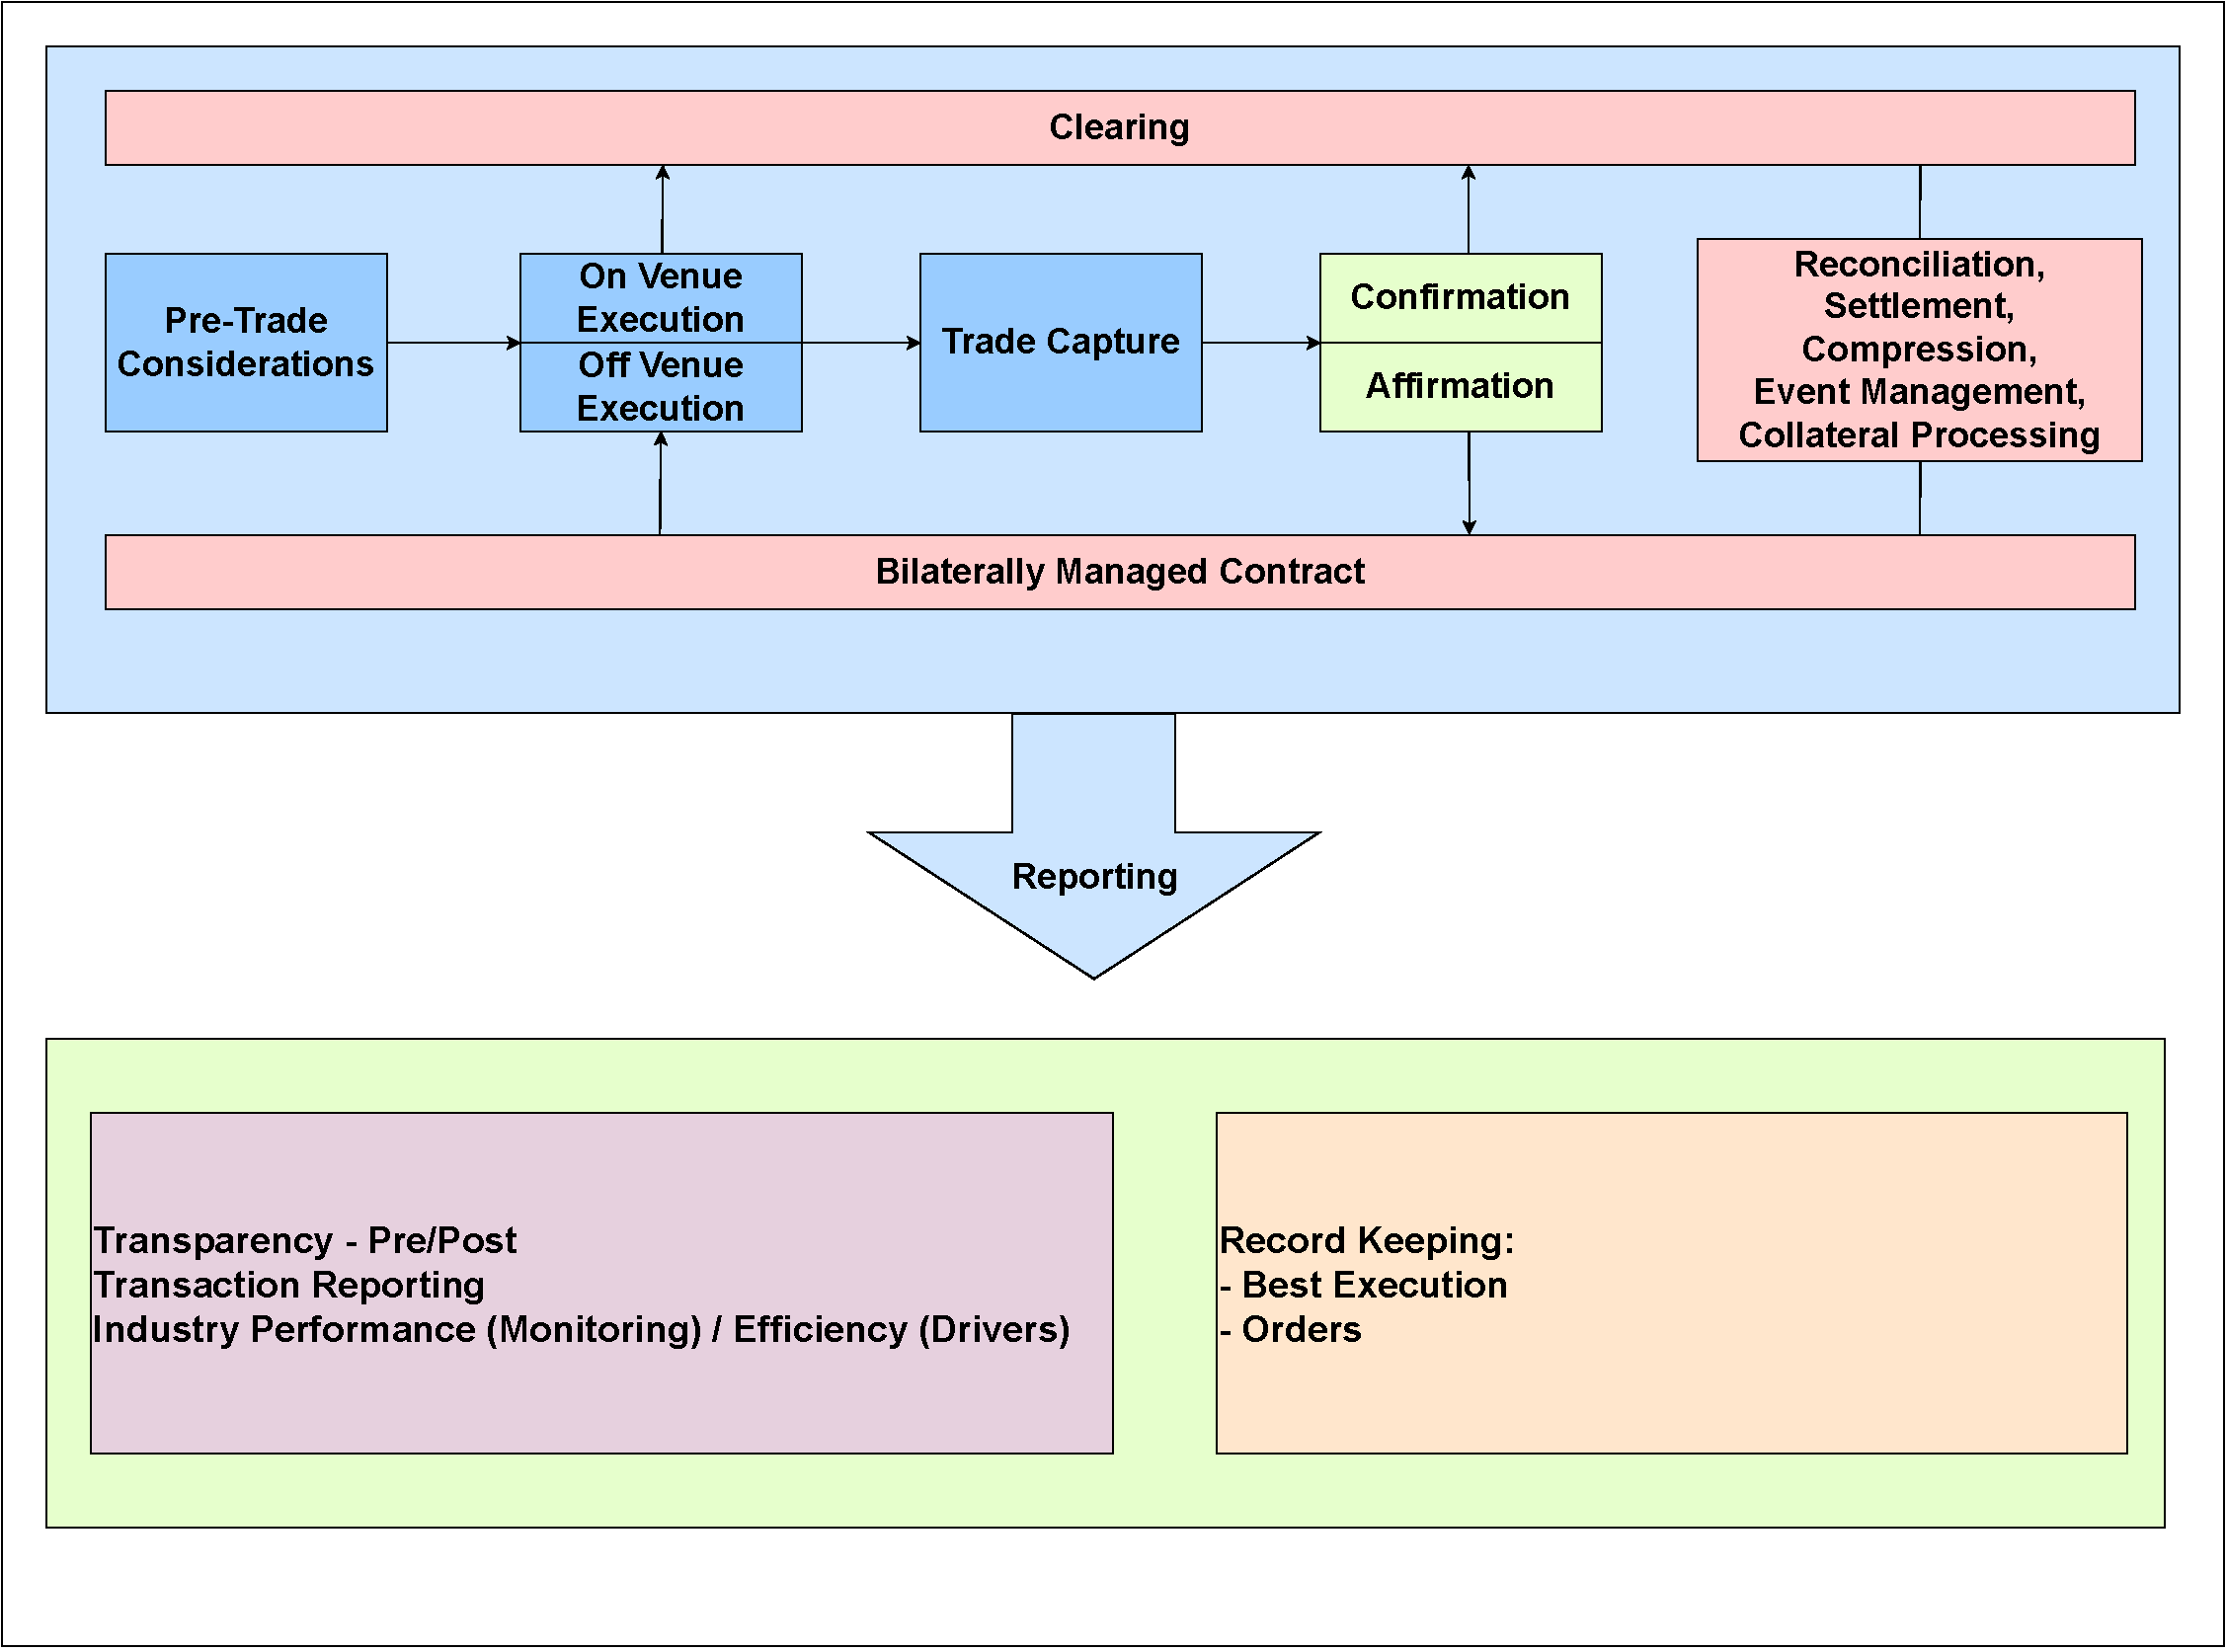
\includegraphics[width=\textwidth]{images/chapter-2/trade-lifecycle.pdf}
    \caption[Derivative Trade Lifecycle]{Adapted from \citep{isda_market_infrastructure}. The steps involved in the lifecycle of a derivative trade as per ISDA definition \citep{isda_market_infrastructure}. Starting with \textit{pre-trade considerations}, parties assess market conditions, risks, and regulatory implications to align their trading strategies. The \textit{trade execution} can either be on-venue, on regulated platforms, or off-venue, directly between parties. Once executed, the trade's details are meticulously captured, followed by a thorough \textit{confirmation and affirmation} process to ensure accuracy and mutual agreement. This leads into a multifaceted phase of \textit{portfolio reconciliation,} \textit{settlement}, \textit{compression} (reducing the number of derivative contracts in a portfolio without altering its net risk profile), \textit{event management}, and \textit{collateral processing}, ensuring both parties have matching records, finalizing the trade, managing lifecycle events, and mitigating credit risks. The \textit{clearing} stage introduces a central counterparty, guaranteeing trade terms and reducing default risks. Comprehensive §\textit{reporting} to authorities ensures transparency and compliance, while diligent \textit{record-keeping} tracks trade history and adherence to best execution practices.
    
    }
    \label{fig:trade-lifecycle}
\end{figure}
\subsection{Collateral}
\label{subsec:collateral}
Collateral refers to the assets or pool of assets that are offered up by one party as a safety net, a guarantee against their contractual obligations \citep{isda_blueprint_collateral_processing}. Collateral can take many forms, ranging from cash and government securities to corporate bonds, equities, or any other asset deemed acceptable by the counterparties. The role of collateral is inherently protective, a safeguard designed to mitigate risk. Should a party default on their obligations, the collateral can be seized by the counterparty to counterbalance any financial loss resulting from the default.

The process of allocating collateral within derivative trades is multifaceted and dynamic. It's not simply a matter of assigning assets at the outset and leaving them be. Rather, it's a continuous recalibration, responding to shifts in the derivative position's market value, changes in the creditworthiness of the counterparties, and the constant ebb and flow of market volatility. This allocation process commences with the posting of an initial margin. This is essentially a percentage of the contract's total value, posted by both parties, acting as the first line of defense against potential market-induced losses.

In addition to the initial margin, counterparties are also required to post a variation margin \citep{IM}. Unlike the initial margin, the variation margin is not static. It's adjusted daily to accurately reflect the ever-changing market value of the derivative contract. Should market movements negatively impact a party's position, they may be called upon to post additional collateral, a process known as a margin call.

Moreover, it's worth noting that in certain circumstances, collateral can be subjected to reuse or rehypothecation. This essentially allows the receiving party to use the collateral for other purposes, such as pledging it for their own derivative trades. This practice, however, is subject to regulatory constraints and must be explicitly permitted in the collateral agreement.

In the world of derivative trades, the accurate valuation of collateral is paramount. From the moment it's posted, the value of collateral must be closely monitored and revalued regularly, often daily, to ensure it remains commensurate with the exposure. The quality of collateral also holds significant weight, with high-quality, highly liquid assets being the preferred choice because they can be swiftly sold if a counterparty default occurs.
\subsection{Collateral Management Challenges}
\label{subsec:collateral_mgmt}
The collateral management process is currently tainted by several challenges, spanning various stages of the lifecycle and posing significant impediments to the efficient operation of financial markets. ISDA provides a breakdown of the most significant elements of friction in the process in their \textit{Blueprint for the Optimal Future State of Collateral Processing} \cite{isda_blueprint_collateral_processing} whitepaper (Figure \ref{fig:collateral_mgmt_steps}). These can be broadly categorised in the following areas:

\begin{itemize}
    \item \textbf{Asset Selection}. The process of asset selection, which determines what constitutes eligible collateral, is guided by a combination of regulatory stipulations and market conventions. However, the ultimate decision on what will be deemed eligible collateral is left to the discretion of the trading partners. This lack of standardization presents a significant challenge. The free-form nature of eligible collateral, typically defined in a Credit Support Annex (CSA), further compounds this issue. Moreover, difficulties arise in determining common definitions for certain asset types, such as high-quality liquid assets (HQLAs) \citep{HQLAs};

    \item \textbf{Margin and Interest Calculation}. The current process of margin and interest calculation is largely manual, making it prone to processing errors. Counterparties independently calculate their interest based on the terms of their agreements, which include agreed rates and day count. This independent calculation often leads to potential discrepancies thereby leading to settlement risk. The manual matching of interest calculation payments and the manual reconciliation process further exacerbate these challenges;

    \item \textbf{Trade Transaction Management}. Mismatched and unmatched trades are primary drivers of disputes in the margin and collateral process. High volumes of new trades and amendments result in daily volatility in portfolios, making the management of these trades a complex task. Portfolio reconciliation is managed on the day following execution, which limits the ability to resolve trade-matching issues prior to issuing margin calls.

    \item \textbf{Record Keeping and Reconciliation}. Record keeping and reconciliation are integral to the collateral lifecycle, but they are also time-consuming and costly. This fragmentation and the resulting inaccuracies pose significant challenges to the efficient operation of financial markets. For instance, the existence of up to 18 trade repositories (entities that centrally collects and maintains the records of OTC derivatives) globally, which are mostly regional or national, limits the scope of trades captured and hampers market transparency \citep{DTCC_trade_repositories}. These repositories are ill-equipped to offer the comprehensive data needed for policymakers to monitor and mitigate systemic risk effectively. As a result, the OTC derivatives market is likely to become less transparent in the future, further complicating record keeping and reconciliation efforts.

    \item \textbf{Operational Challenges}. The operational challenges associated with the collateral lifecycle are also significant. Principals often face difficulties in releasing assets as collateral due to regulatory rules and operational challenges. When certain assets are used as collateral, it involves physical movements of those assets to 3rd party accounts. This physical movement of assets incurs significant costs and operational overheads.

    \begin{figure}[!h]
        \centering
        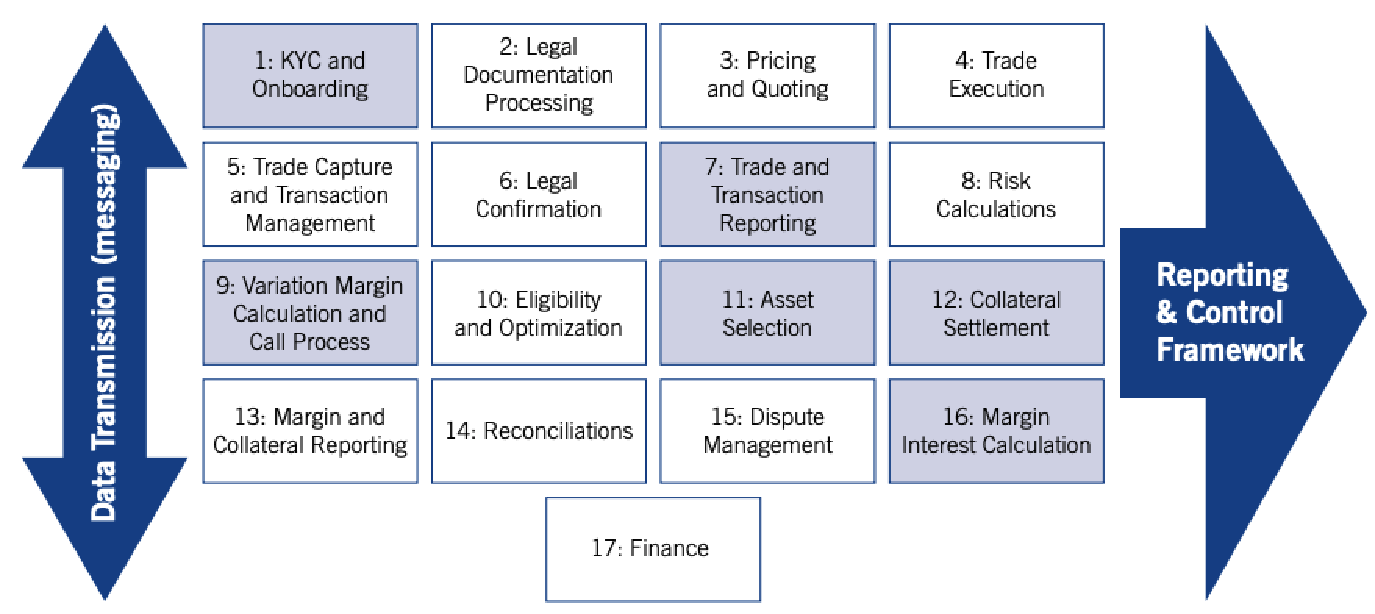
\includegraphics[width=\textwidth]{images/chapter-2/collateral-challenges.pdf}
        \caption[Collateral Management Processes]{Reproduced from \cite{isda_blueprint_collateral_processing}. Stages of Collateral Management: Highlighted steps are discussed in the ISDA Blueprint \citep{isda_blueprint_collateral_processing}. \textit{KYC \& Onboarding} often grapple with intricate due diligence requirements and data inconsistency across global jurisdictions. \textit{Trade and Transaction Reporting} faces the challenge of ensuring timely and accurate data submissions amidst diverse regulatory standards.\textit{ Variation Margin Calculation and Call Process} can be complex due to fluctuations in market prices and differing contractual terms. \textit{Asset Selection} confronts the dilemma of balancing optimal returns with counterparty acceptability and liquidity constraints.\textit{ Collateral Settlement} experiences delays due to multi-party involvement and reconciliation discrepancies. Lastly,\textit{ Margin Interest Calculation} struggles with diverse rate agreements and the intricacies of time-bound computations.}
        \label{fig:collateral_mgmt_steps}
    \end{figure}
    
\end{itemize}

\section{Industry and Regulatory Standards}
\label{sec:industry_approach}

\subsection{ISDA Common Domain Model}
\label{subsec:cdm}
The ISDA Common Domain Model (CDM) \citep{isda_cdm_factsheet} is a groundbreaking initiative aimed at bringing uniformity to the financial markets. It addresses the challenges posed by the increasing intricacy of the industry and the pressing need for streamlined operations. The model functions as a comprehensive framework that is both "machine-readable" and "executable." In simpler terms, "machine-readable" means that the data and rules within the CDM can be easily understood by computers without human intervention. "Executable" means that the model can automatically carry out transactions and processes, further reducing manual effort. Being an open-source project, the CDM is freely accessible and can be modified to suit the specific needs of different organizations in the financial sector. This adaptability is particularly beneficial for industry participants looking for tailored solutions. 

One of the primary objectives of the CDM is to enhance operational efficiency in financial markets. It does this by setting a digital standard for various trading activities and events. This uniform standard makes it easier for different companies and platforms to interact with each other, thereby minimizing the discrepancies that often require time-consuming reconciliation.

Transparency is another cornerstone of the CDM. It ensures that regulatory bodies and market participants are aligned, which is crucial for consistent reporting to authorities. The model is built on foundational design principles such as "abstraction-based normalization," which means simplifying complex elements to their most basic forms; "composability," or the ability to combine different components seamlessly; and "modularization," which allows for easy updates and modifications. These principles contribute to the robustness and flexibility of the CDM.

Governed by a structured set of guidelines, the CDM is applicable to a broad spectrum of financial products, including but not limited to Over-The-Counter (OTC) derivatives and cash securities. The model comprises various elements, including the publicly accessible ISDA CDM Distribution \citep{cdm_distribution_github}, the specialized Rosetta Domain-Specific Language (DSL) \citep{rosetta_dsl}, and a supportive ecosystem of applications built on the CDM framework \citep{applications_cdm}.
\subsection{ISDA Create}
\label{subsec:isda_create}
ISDA Create \citep{isda_create_factsheet} is a digital platform developed to automate the negotiation and execution of documentation used in the derivatives and securities financing markets. By transitioning from manual, paper-based processes to a more streamlined digital approach, ISDA Create aims to enhance efficiency and reduce the time taken to finalize agreements. The platform provides users with the ability to negotiate and execute multiple documents simultaneously, offering a centralized location for storage and access. This centralized approach simplifies the tracking of negotiations, document version control, and the overall management of legal agreements. Additionally, ISDA Create supports the integration of standardized data structures, facilitating easier data extraction and analysis. 

\subsection{ISDA Clause Library}
\label{subsec:clause_library}
The ISDA Clause Library \citep{isda_clause_library_factsheet} is an initiative aimed at providing clarity and consistency in the documentation of derivatives trade agreements. Recognizing the complexities and nuances inherent in these contracts, the library offers a structured approach to categorizing and defining standard clauses used in ISDA documentation. By doing so, it facilitates a more streamlined negotiation process, reducing ambiguities and potential misunderstandings between parties. The library serves as a reference tool, enabling legal professionals and contract negotiators to quickly identify and understand the implications of specific clauses. This systematic approach not only simplifies the drafting process but also aids in ensuring compliance with regulatory requirements.
\subsection{Industry Participants}
\label{subsec:industry_participants}
The drive from ISDA towards increasing standardization and digitization of the derivative trading lifecycle has been echoed by both established financial institutions and emerging startups, leveraging cutting-edge technologies like AI and blockchain. J.P. Morgan, a banking behemoth, has been actively exploring the potential of blockchain in streamlining derivative transactions. Their Liink product (formerly Interbank Information Network or IIN) aims to reduce friction in the information exchange process, ensuring smoother and more efficient derivative trades \citep{jpm_liink}. Barclays, another banking giant, has also shown interest in blockchain's potential to revolutionize the derivative trading landscape. They believe that the technology can address the challenges of transparency and efficiency that have long plagued the sector \citep{barclays}. On the startup front, Digital Asset is making waves with its smart contract language, DAML, which seeks to automate and digitize complex derivative contracts, making them more accessible and transparent \citep{daml}. Clause \citep{clause_startup} is another innovative startup that integrates AI and blockchain to automate real-time derivative contract performance. Their platform can interpret and execute clauses in derivative contracts, ensuring that all parties adhere to the agreed terms. Lastly, Komgo \citep{komgo_startup} is a blockchain-based platform that focuses on commodity trade finance, a subset of derivative trading. By offering a decentralized solution, Komgo aims to reduce fraud and operational errors, ensuring a more secure and efficient trading environment.

\section{Blockchain}
\label{sec:blockchain}
Blockchain is a decentralized and distributed ledger technology that allows multiple participants to maintain a shared and tamper-evident record of transactions or information in a secure and transparent manner \citep{morini2016blockchain}. It was originally introduced as the underlying technology for cryptocurrencies like Bitcoin, but its potential applications have expanded beyond digital currencies.

At its core, a blockchain is a chronological chain of blocks, where each block contains a batch of validated transactions or data. Each block is linked to the previous one through a cryptographic hash, creating a chain of information that is extremely difficult to alter. Throughout the rest of this work we use the term "immutable" to describe this chain, however it's important to note that blockchain blocks can technically be changed. However, any alteration to a previous block would become immediately evident when the cryptographic hashes are checked, requiring the modification of all subsequent blocks. This makes the blockchain highly resistant to tampering and ensures the integrity of the data.

Blockchain is particularly suited to address the challenges encountered in the collateral management lifecycle described in section \label{sec: infratrcture_challenges}. In particular,

\begin{itemize}
    \item \textbf{Asset Selection}. By incorporating blockchain technology, the process of asset selection can be significantly standardised. This is achievable by establishing a decentralised protocol for defining eligible collateral, thereby eliminating the discretion and free-form nature of the selection process. This protocol could also include a consensus mechanism to agree on definitions for asset types such as HQLAs, reducing misunderstandings and potential disputes.

    \item \textbf{Margin and Interest Calculation}. Blockchain's smart contracts, which are programmable contracts that automatically execute when certain conditions are met, could automate the manual, error-prone process of margin and interest calculation. By setting the terms of agreements, including rates and day count, as the conditions in the smart contract, the calculations would be automatically performed and agreed upon by all parties involved, thereby eliminating discrepancies and reducing settlement risks.
    
    \item \textbf{Trade Transaction Management}. Blockchain's immutability and real-time transaction records can significantly enhance trade transaction management. By storing every new trade and amendment on the blockchain, all parties can monitor the portfolio volatility and address trade-matching issues immediately, rather than waiting for the following day. This would minimise mismatches and unmatched trades, reducing the disputes in the margin and collateral process.
    
    \item \textbf{Record Keeping and Reconciliation}. With blockchain technology, record keeping and reconciliation could be streamlined and automated. Each transaction and adjustment made during the collateral lifecycle would be recorded in real-time on the blockchain. This permanent, transparent ledger would provide a single source of truth for all participants, thus eliminating data fragmentation, reducing the inaccuracies in trade reporting, and cutting down the time and cost of reconciliation.
    
    \item \textbf{Operational Challenges}. The use of blockchain could also mitigate the operational challenges involved in the collateral lifecycle. The movement of assets used as collateral could be represented as token transfers within the blockchain, bypassing the need for physical transfer of assets. This could expedite the process, reduce costs, and make it easier to comply with regulatory rules. By tokenizing assets, principals could also easily release assets as collateral, enhancing operational efficiency. The benefits of efficient release and re-allocation of collateral are described in detail in Section \ref{subsec:benefits_financial}.
\end{itemize}
\subsection{Smart Contracts}
\label{sec:smart_contracts}
The term "smart contract" was first coined in the 1990s by computer scientist and cryptographer Nick Szabo \citep{szabo1997formalizing}, long before the rise of blockchain technology, as we know it today. Szabo envisaged smart contracts as computerized transaction protocols that execute the terms of a contract, aiming to deliver highly efficient, automated solutions to contract law.

Today, in the backdrop of blockchain technology, the term "smart contracts" has become used to refer to programmable, self-executing, and self-enforcing protocols that run on the blockchain. They are essentially predefined rules and conditions encapsulated in the form of a digital contract. Once these predefined conditions are met, the smart contract automatically triggers a transaction or a specific action, making the whole process tamper-evident and leaving no room for default.
\subsubsection{Smart Legal Contracts}
\label{subsec:smart_legal_contracts}
Taking the concept of smart contracts a step further are "smart legal contracts" – these are conventional legal contracts interwoven with smart contract functionalities \citep{ruhl2021smart}. A smart legal contract is essentially a legal agreement that has some or all terms and conditions represented and executed by software. These contracts are not only legally binding agreements but also contain provisions that are capable of being automated and carried out by a machine, providing the best of both worlds – the solidity of legal contracts and the automation of smart contracts.
\subsubsection{Smart Derivative Contracts}
\label{subsec:smart_derivative_contracts}
One specific application of smart contracts in the finance industry is the emergence of "smart derivative contracts" \citep{clack2019smart}. Smart derivative contracts have the potential to revolutionize the derivatives market by embedding the terms of a derivative contract on a blockchain. These self-executing contracts can automate the life cycle of a derivative trade, from creating the contract, performing valuations, managing margins, and all the way to the final settlement.

When applied to collateral management in derivatives trading, smart derivative contracts can automate collateral posting and maintenance, which are often complex and resource-intensive processes. These contracts can be programmed to monitor the value of the collateral and automatically issue margin calls when necessary. The blockchain's immutability ensures that the smart derivative contracts are tamper-evident and their execution can be audited, thereby improving the security and transparency of the process. This use of blockchain and smart derivative contracts promises to transform collateral management, significantly reducing the risks, costs, and inefficiencies associated with the process.
\subsection{Bitcoin Satoshi Vision}
\label{subsec:bsv}
Bitcoin Satoshi Vision (BSV) is a cryptocurrency and blockchain network that emerged from a hard fork split from Bitcoin Cash (BCH) in November 2018 \citep{bsv_home}. It was created in response to disagreements within the Bitcoin Cash community over proposed changes to the protocol. BSV proponents, led by Craig Wright and Calvin Ayre, sought to adhere more closely to what they consider to be the original vision of Bitcoin's anonymous creator, Satoshi Nakamoto. This vision encompasses principles of larger scalability, minimal transaction fees, and robust data handling, making BSV uniquely suited to address the challenges in the collateral management lifecycle. In particular, the benefits offered by BSV in the collateral management process become even more evident when compared to alternative distributed ledger platforms such as Ethereum Bitcoin:

\begin{itemize}
    \item \label{item:scalability} \textbf{Scalability}. BSV's main advantage is its scalability, which is primarily achieved by significantly increasing the block size limit as compared to Bitcoin and Ethereum. The original Bitcoin and Ethereum networks have opted for smaller block sizes (1 MB, fixed-size blocks for Bitcoin \citep{btc_block_size_limit} and variable-sized blocks for Ethereum --- up to a ceiling of 30 million "gas" units \citep{eth_block_size}, where "gas" is the unit of measurement for computational effort that is required to perform various operations, such as executing smart contracts, making transactions, or storing data \citep{eth_gas}) to maintain decentralization and security. Smaller block sizes are easier for individual nodes to process, thereby encouraging more participants and maintaining the decentralized nature of the blockchain. However, the trade-off is a limited throughput of transactions, which can slow down the network and increase transaction fees during periods of high demand \citep{singh2020computing}. BSV, on the other hand, has decided to prioritize scalability by allowing much larger block sizes (up to 4GB at the time of writing \citep{bsv_block_size}), aiming to accommodate more transactions per block. This enables quicker processing of transactions, creating a responsive system that is ideal for managing daily portfolio volatility and facilitating trade transactions. Fixed block sizes are generally used as a compromise between scalability and network health; variable block sizes could lead to inconsistencies in block propagation and validation times, potentially compromising the security and integrity of the network \citep{singh2020computing}.

    \item \textbf{Data Handling}. BSV provides robust data handling capabilities, allowing for comprehensive transaction data to be stored directly on the chain. While Ethereum also supports data storage, its higher transaction fees for complex data operations may limit efficiency. BSV's capabilities ensure an efficient, transparent, and immutable record of collateral lifecycle events, which dramatically improves record keeping, reconciliation, and reporting accuracy.
    
    \item \label{item:smart_contracts} \textbf{Smart Contracts}. BSV's smart contracts offer an economical approach to automating processes in the collateral management lifecycle. Unlike Ethereum or Bitcoin's smart contracts, which can incur high gas fees, BSV has significantly lower transaction costs, though it is not entirely without fees --- at the time of writing (5th September 2023), the average transaction cost is \$0.81 on Ethereum \citep{eth_tx_fee}, \$1.40 on Bitcoin \citep{btc_tx_fee} and \$0.00000367 on BSV \citep{bsv_tx_fee}. This makes it more cost-effective for executing complex automation tasks, such as margin and interest calculations and asset selection. Additionally, BSV, similarly to Bitcoin, incorporates specific safeguards such as opcode limits and script size restrictions to minimize the risk of "runaway processes" like infinite loops \citep{btc_limits_safeguards}. This contrasts with Ethereum, where the presence of high gas fees often acts as a de facto limitation against such inefficiencies but doesn't provide built-in safeguards in the protocol \citep{eth_loops}. BSV's approach ensures a more streamlined and reliable experience for executing smart contracts, without relying solely on transaction costs as a deterrent against poorly optimized code.
    
    \item \textbf{Micropayments}. BSV's low transaction fees make it highly effective for micropayments, allowing for flexible interest payment schedules and streamlined settlements. This directly contrasts with Ethereum, where high gas fees make small transactions economically inefficient. BSV's affordability in this context significantly minimizes the need for manual reconciliation processes, such as matching transactions, verifying records, and resolving discrepancies, thereby reducing both time and labor costs.
    
    \item \textbf{Tokenization}. Both BSV and Ethereum platforms offer the capability to tokenize assets, thereby streamlining the collateral management lifecycle. Tokenization on these platforms eliminates the need for physical asset transfer, enhancing operational efficiency. However, the two differ in terms of transaction costs. BSV offers a more cost-effective solution for asset tokenization and transfer, while Ethereum, although equally functional in allowing tokenization, comes with higher transaction fees \citep{di2020tokens}. This makes BSV a more economical choice for businesses looking to manage operational challenges in collateral management without sacrificing functionality.
\end{itemize}
\subsubsection{UTXOs}
\label{subsec:utxos}
In the BSV blockchain, the Unspent Transaction Output (UTXO) model serves as the cornerstone for enabling transactions. Unlike traditional account-based models, where the state of an account is updated continuously, UTXOs are discrete data units that represent a specific amount of cryptocurrency \citep{antonopoulos2014mastering}. Each UTXO consists of its value in satoshis (the smallest unit of a Bitcoin) and a ScriptPubKey --- a cryptographic script that outlines the conditions for spending that particular UTXO. UTXOs are created as outputs from transactions and can be thought of as virtual "coins" that can be consumed or spent in subsequent transactions. When a UTXO is spent, it becomes an input for a new transaction, and the process creates new UTXOs as outputs, which in turn can be spent in the future.

The ScriptPubKey associated with each UTXO specifies the "locking script" that must be "unlocked" by a corresponding "unlocking script" or ScriptSig for the UTXO to be spent. Different types of ScriptPubKeys exist to facilitate various transaction types. Pay-to-Public-Key-Hash (P2PKH) \citep{p2pkh} is one of the most common types, designed for simple, one-to-one transactions. In a P2PKH output, the ScriptPubKey locks the UTXO with the hash of the recipient's public key. To spend it, the recipient must provide both the public key and a digital signature that proves ownership of the corresponding private key.

Pay-to-Script-Hash (P2SH) \citep{p2sh} offers more complexity and flexibility, enabling outputs to be locked with a hash of a script rather than a public key. P2SH allows for more complicated locking conditions, like multi-signature requirements or time-locked releases. In a P2SH transaction, the person who sets the conditions is not necessarily the one who fulfills them. This type enables functionalities like multi-signature wallets, where multiple parties must sign off on a transaction, or smart contracts that execute automatically under predetermined conditions.

Together, these UTXO features and ScriptPubKey types make up the rich ecosystem of transaction possibilities in the BSV blockchain, offering both robust security measures and versatile programmability.

\begin{figure}
    \centering
    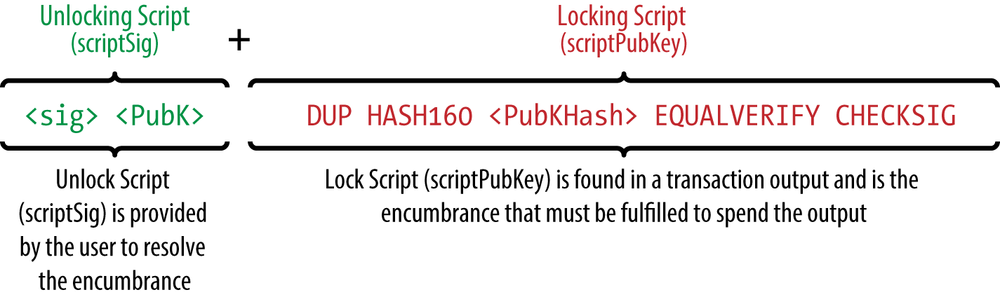
\includegraphics[width=\textwidth]{images/chapter-2/utxo.png}
    \caption[Unspent Transaction Output]{Reproduced from \citep{antonopoulos2014mastering}. Unspent Transaction Output, with a focus on the ScriptSig and ScriptPubKey components. ScriptSig serves as the 'unlocking script,' providing the necessary credentials to spend a UTXO. The ScriptPubKey acts as the 'locking script,' setting the conditions under which the UTXO can be spent. Together, these cryptographic scripts form the basis for secure and programmable transactions on the BSV blockchain.}
    \label{fig:utxo}
\end{figure}



\subsubsection{sCrypt}
\label{subsec:sCrypt}
sCrypt \citep{scrypt_home} is a high-level scripting language purpose-built for writing smart contracts on the BSV blockchain. It was conceived as a more developer-friendly alternative to Bitcoin's low-level scripting language, Bitcoin Script. While Bitcoin Script has proven to be highly secure and robust, it is also complex and cumbersome for developers, especially those new to blockchain development. To address this, sCrypt was developed to provide a statically-typed, C-style syntax that is both expressive and familiar to developers, thereby improving the readability, development efficiency, and bug detection in BSV smart contracts.

In our project to tokenize collateral assets on BSV, we are using sCrypt for several key reasons:

\begin{itemize}
    \item \textbf{Efficiency and Readability}. The syntax of sCrypt is similar to popular programming languages such as TypeScript \citep{typescript_home}, making it easier to write, read, and maintain. This improves efficiency and reduces the potential for errors in the development process.

    \item \textbf{Security}. sCrypt is engineered to tap into the native security protocols of Bitcoin Script by directly cross-compiling from its high-level language to Bitcoin Script. Through the process of cross-compilation via Typescript, sCrypt allows for the development of smart contracts that are not only secure but also reliable and robust. This direct translation ensures that the smart contracts are tightly integrated with Bitcoin's established security features, guaranteeing the integrity of our tokenized collateral assets without introducing extraneous vulnerabilities.
    
    \item \textbf{Static Typing}. sCrypt is a statically typed language, which enables the detection of many errors at compile-time rather than at run-time. This is particularly important in blockchain development where contracts are immutable once deployed.
    
    \item \textbf{Built for BSV}. sCrypt is specifically designed for the BSV blockchain. This ensures smart contracts can fully leverage the unique features of BSV, such as its scalability and microtransaction capabilities, which are integral to managing tokenized collateral assets at scale.
\end{itemize}
\subsection{Oracles}
\label{subsec:oracles}
Oracles, within the context of blockchain and smart contract technologies, serve as intermediaries that provide the bridge between blockchain systems and the external world \citep{al2020trustworthy}. They relay real-world data to smart contracts on the blockchain, enabling these decentralized applications to interact and integrate with off-chain data and systems. Given that blockchains are deterministic systems, they can't directly interact with the external world because they operate based on pre-defined rules and consensus mechanisms that ensure security and immutability within the network. Since blockchains are designed to be isolated systems to maintain their integrity and trustworthiness, any interaction with external data sources poses the risk of introducing vulnerabilities or inaccuracies. Thus, they need a trusted channel to provide them the necessary data, and that's where oracles come in.

Oracles can be of various types, such as input oracles, output oracles, cross-chain oracles, and compute-enabled oracles \citep{types_oracles}. Input oracles fetch real-world data and deliver it to the blockchain for smart contracts to use. Output oracles, on the other hand, enable smart contracts to dispatch instructions to external systems, prompting them to carry out specific actions. Cross-chain oracles facilitate data and asset movement between different blockchains, thus enabling interoperability. Compute-enabled oracles provide off-chain computation capabilities that are impractical to perform on-chain due to various constraints.

Oracles can significantly enhance the efficiency and robustness of collateral management systems in several ways:

\begin{itemize}
    \item \textbf{Real-time Price Feeds} \citep{Decentralized_Data_Feeds}. The foundation of collateral management is the accurate valuation of collateral assets. Oracles, especially input oracles, deliver real-time market data relating to the prices of assets that serve as collateral in smart contracts. As an example, in scenarios where a specific cryptocurrency or token is put forth as collateral, an oracle can supply its latest market price, ensuring that the valuation of the collateral is as precise as possible. In the context of decentralized finance (DeFi), such data streams can stimulate automated reactions when prices hit predetermined thresholds - for instance, it may launch a margin call when the collateral's value dips below a certain level, thus ensuring prompt action and prevention of potential risks.

    \item \textbf{Risk Management} \citep{volatility_oracles}. Proficient collateral management hinges on robust risk management protocols, and oracles play an instrumental role in this area. They have the capacity to supply data concerning the volatility and liquidity of assets under consideration as collateral. This information aids in assessing associated risks - for example, an asset with high volatility brings with it a higher risk of a sharp decline in its value, which could result in the collateral's value being insufficient. Oracles deliver real-time data feeds that can support these risk assessments and guide better informed, proactive decision-making.
    
    \item \textbf{Automation of Collateral Calls}. Oracles and smart contracts together contribute to automating collateral calls, each serving distinct roles within the system. In this setup, oracles function as real-time data feeds that continuously monitor market conditions and the valuation of the counterparty's collateral. When these oracles detect that the market circumstances have changed unfavorably, thereby devaluing the collateral to an insufficient level, they pass this critical information to the smart contract. On the other hand, the smart contract holds the pre-defined logic for executing a collateral call based on the information received from the oracle. It determines if the collateral devaluation warrants an automatic call, calculates the additional amount of collateral required, and then triggers the collateral call to the counterparty. The smart contract also facilitates the secure, trustless transaction of posting additional collateral, making the entire process more efficient and transparent. This is the use case the we propose as part of system described in Chapter \ref{ch:solutionArchitecture}.

 
    \item \textbf{Regulatory and Compliance Checks}. Oracles can play a critical role in not just retrieving data related to regulatory obligations and compliance checks, but also in ensuring that smart contracts remain up-to-date with real-time changes in regulations and industry-standard practices. This is especially significant given that regulations and compliance standards are often subject to change, and smart contracts, once deployed, are immutable by nature \citep{zheng2020overview}. To address this, smart contracts must be designed with "upgradability" in mind, allowing for the modification of their logic without requiring the redeployment of the entire contract. Various techniques exist to achieve upgradability, such as using external libraries, data separation, or the proxy pattern \citep{meisami2023comprehensive}. In particular, the proxy pattern \citep{proxy_pattern} is a technique wherein the main smart contract delegates its logic to another contract (often termed the "implementation contract"). The proxy contains the state variables and remains consistent, while the logic and data manipulation are conducted in the implementation contract. When regulations change, a new implementation contract can be deployed and linked to the existing proxy, ensuring that compliance-related data is always current and that collateral evaluation criteria align with the latest regulatory requirements. At the time of writing and to the best of our knowledge, no specific  oracles solely dedicated to providing information about standards and regulations exist. However we envision, and in fact suggest, ISDA launching its own oracle service to provide requirements about, for example, the eligibility of different types of collateral \citep{cdm_website}. 
    
    \item \textbf{Cross-chain Interoperability} \citep{crosschain_oracles}. In a context where multiple blockchains are in operation, the same asset could exist on several chains. Cross-chain oracles in such scenarios can be invaluable, enabling smart contracts to identify and engage with these assets across different chains. This significantly improves the flexibility and scope of the collateral management process.
    
    \item \textbf{Settlement and Reconciliation}. Oracles can also expedite the settlement and reconciliation process inherent to collateral management. Output oracles, for instance, can engage with traditional banking systems to initiate payments based on the stipulations of a smart contract, thereby seamlessly aligning traditional and decentralized finance systems \citep{tradfi_defi_oracles}.
\end{itemize}

\section{Asset Tokenisation}
\label{sec:asset_tokenisation}
Asset tokenization is the process of converting the rights to a physical or intangible asset into a digital token on a blockchain. These tokens can represent a wide variety of financial instruments, including equities, bonds, real estate, commodities, and even artworks or intellectual property. There are several types of tokens, each with their unique properties and applications \cite{isda_tokenisation_models}. Table \ref{tab:tokenisation_models} provides a breakdown of the distinguishing features of each model.

\begin{itemize}

    \item \textbf{Registered Tokens} \citep{registered_tokens}. These tokens have an identity layer. Ownership of these tokens is tied to a specific identity, which can be verified against a registry. This is particularly useful for assets where legal and regulatory compliance is crucial (Figure \ref{subfig:registered}). The first ever digital bond, denominated in GBP, issued by the European Investment Bank lies in this category \citep{eib_bond}.

    In the Registered model, ownership of tokenised assets is tied to a specific identity stored in a register controlled by a \textit{Registrar} entity. The Registrar and the \textit{Issuer} of the tokens could coincide. When they do not, the Issuer submits instructions to the Registrar when issuance operations have to be performed, as well as transferring the ownership rights of the tokenised securities to the Participants in the network. Transfer operations are performed by the Participants by issuing transfer instructions to the Registrar. It is important to highlight the fact that in this scenario the power to update and rectify entries in the registers lies exclusively with the \textit{Registrar}, the Issuers and Participants can simply communicate the actions they want to perform. Another important aspect to consider is that in this scenario the tokens merely represent evidence of rights, they are not assets in their own right, and modifying the state of the register simply involves updating the token balances of specific participants. Note that two registers are present: the first, on-chain register stores the mapping between public keys and tokens, i.e. the holding relationships; the second, off-chain register maps public keys to real-world identities. The Registrar also keeps an offline business continuity record, essentially replicating the on-chain records, to ensure operations can proceed in case of network disruptions.
    
    \item \textbf{Bearer Tokens} \citep{bearer_tokens}. These are tokens that grant ownership to whoever holds them, much like cash or certain types of bonds. They don't have an embedded identity layer that verifies the owner's identity. Whoever controls the private key controls the asset (Figure \ref{subfig:bearer}). Stablecoins (dollar-pedgged digital coins) such as USDT \citep{usdt} and USDC \citep{usdc} fall into this category.

    In the Bearer model, the tokens are intangible assets in their own right and ownership of tokenised assets relies exclusively on the control of the tokens themselves. In this scenario, no Registrar is needed; the Issuer simply creates the tokens and transfers ownership to the Participants, which are then fully responsible for administering the assets. It is important to highlight that in this scenario the token holder has exclusive control, meaning the token holder has additional operational burdens as well as increased exposure to risk. Moving funds requires updating ownership of the asset themselves (meaning that once the asset is transferred, associated rights and control over it now belong to the new holder, increasing risks related to irreversibility of transactions in case of errors).

    \item \textbf{Claim Tokens} \citep{claims_tokens}. These tokens represent a claim or a right against an asset, rather than the asset itself. They're often used in debt issuance or other types of contractual agreements where one party has a claim against another (Figure \ref{subfig:claims}) The Depository Trust \& Clearing Corporation's (DTCC) Ion Project, a blockchain-based alternative settlement engine, falls into this category \citep{project_ion}.

    In the Claims model, a third-party Operator is responsible for running and maintaining the blockchain system, while also providing the rules for operating within the system. The Claims model resembles the Registered model, however we note a few key differences. Firstly, there is no additional identity layer, ownership is fully determined within the boundaries of the blockchain system by means of cryptography (mapping between public keys and token representations). Secondly, the Issuer and Operator cannot coincide: the Issuer is exclusively responsible for granting ownership rights to the Participant while the Operator's only responsibility is to run the network. Lastly, Participants are directly interacting with each other: ownership changes are still reflected by updates to a ledger of balances, however these are performed directly by Participants by interacting with smart contracts deployed by the Operator (and whose specifications are defined in the system rules). Overall, the Claims model is more flexible than the Registered model in the array of underlying assets it can represent, however this also introduces an extra layer of complexity as the claims must be exercised through appropriate legal channels and contractual arrangements.
    
\end{itemize}


\begin{figure}
     \centering
     \begin{subfigure}[b]{0.8\textwidth}
         \centering
         \begin{minipage}[b][8cm][c]{\linewidth} % Adjust the height (4.5cm) as needed
             \centering
             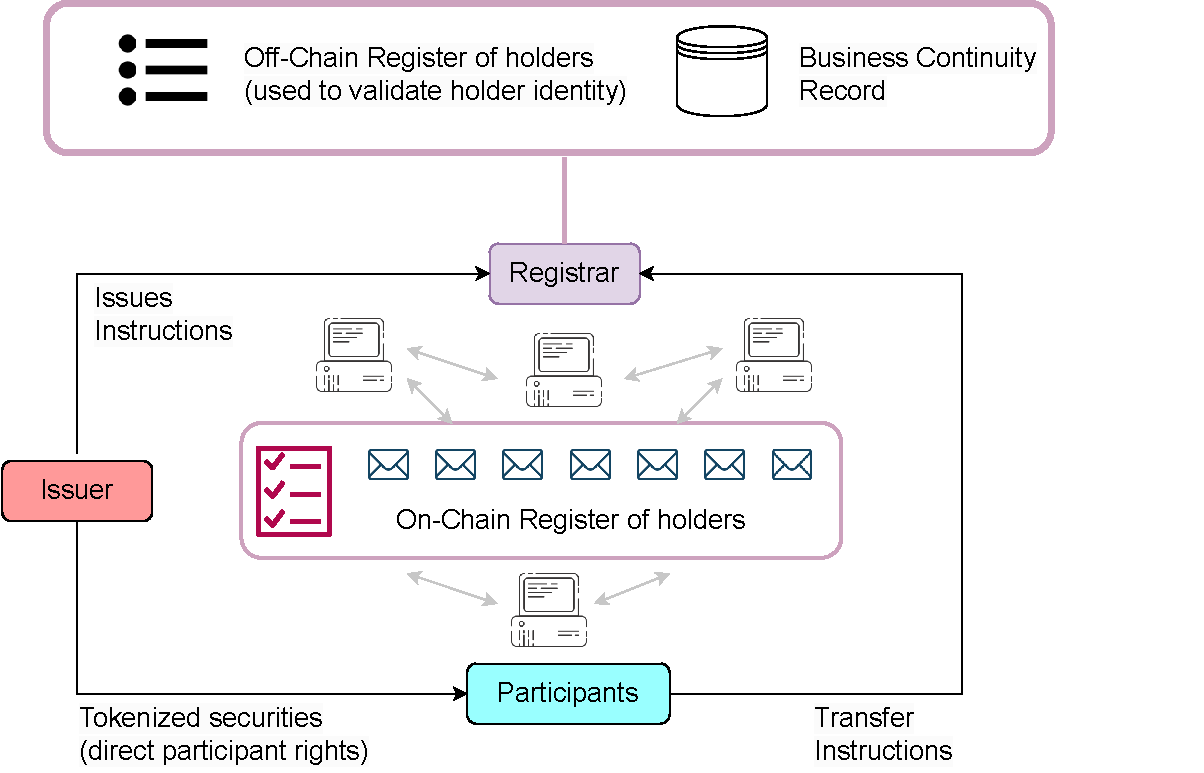
\includegraphics[width=0.8\linewidth]{images/chapter-2/registerd_custom.drawio.pdf}
             \caption{Registered}
             \label{subfig:registered}
         \end{minipage}
     \end{subfigure}
     \\
     \begin{subfigure}[b]{0.7\textwidth}
         \centering
         \begin{minipage}[b][8cm][c]{\linewidth} % Adjust the height (4.5cm) as needed
             \centering
             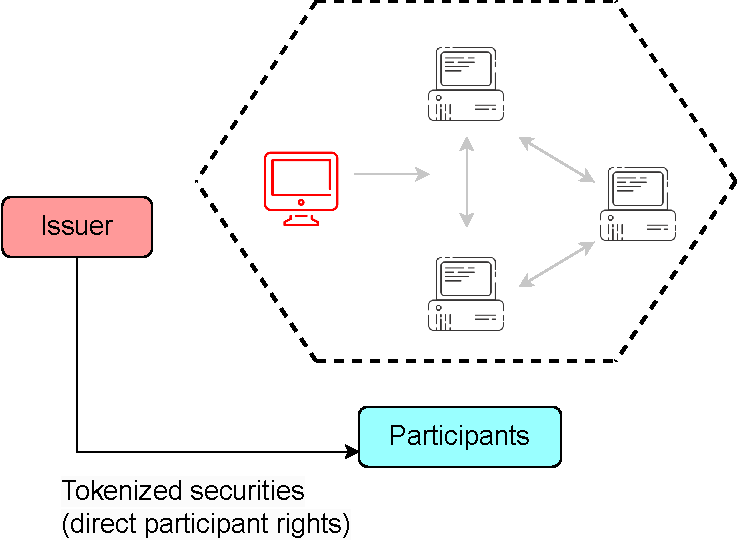
\includegraphics[width=0.8\linewidth]{images/chapter-2/bearer_custom.drawio.pdf}
             \caption{Bearer}
             \label{subfig:bearer}
         \end{minipage}
     \end{subfigure}
     \\
     \begin{subfigure}[b]{0.7\textwidth}
         \centering
         \begin{minipage}[b][7cm][c]{\linewidth} % Adjust the height (4.5cm) as needed
             \centering
             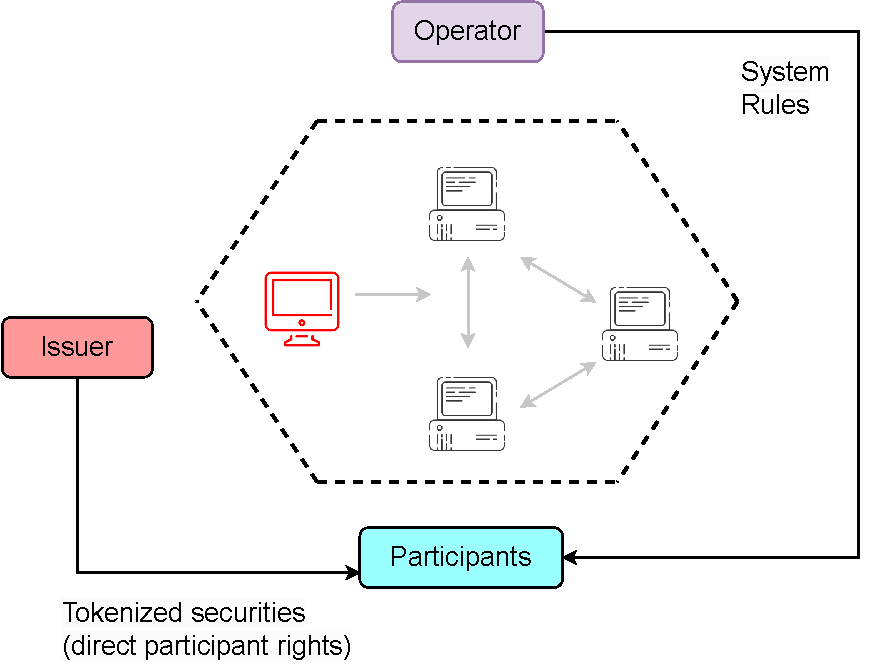
\includegraphics[width=0.8\linewidth]{images/chapter-2/claims_custom.drawio.pdf}
             \caption{Claims}
             \label{subfig:claims}
         \end{minipage}
     \end{subfigure}
    \caption[Asset tokenisation models]{Adapted from \citep{tokenovate_tokenisation_models} \footnotemark. Three asset tokenisation models showing roles of \textit{Issuers}, \textit{Registrars}, and \textit{Participants} in the network: Registered (\ref{subfig:registered}), Bearer (\ref{subfig:bearer}), and Claims (\ref{subfig:claims}) models.}
    
    \label{fig:three graphs}
\end{figure}
\footnotetext{This image is reproduced with permission from Tokenovate Ltd.}


\renewcommand\tabularxcolumn[1]{m{#1}}% for vertical centering text in X column
\begin{table}[]
    \centering

    \begin{tabularx}{\textwidth} { 
           >{\centering\arraybackslash}X 
           >{\centering\arraybackslash}X
           >{\centering\arraybackslash}X
           >{\centering\arraybackslash}X
           >{\centering\arraybackslash}X
           >{\centering\arraybackslash}X  }
         \toprule[1.5pt]
         \textit{Tokenisation Model} & \textit{Description} & \textit{Control} & \textit{Traits} & \textit{Transfer Mechanism} & \textit{Examples} \\
         \midrule[1.5pt]
         
         Registered & \vspace{10pt} Rights determined by reference to a register controlled by Registrar \vspace{1pt} & Registrar has powers to update/rectify entries & Mere data/evidence of rights & Updating token balances & First EIB \href{https://www.eib.org/en/press/all/2023-030-eib-issues-its-first-ever-digital-bond-in-british-pounds}{Digital Bond in Sterling} \citep{eib_bond} \\
    
         \hline

         Bearer & \vspace{10pt} Rights determined by reference to exclusive control of tokens \vspace{10pt} & Token holder has exclusive control & Intangible asset in its own right & Transfer of control of token & \href{https://tether.to/en/why-tether}{USDT} \citep{usdt}, \href{https://www.circle.com/en/usdc}{USDC} \citep{usdc} \\ 

         \hline

         Claims & \vspace{10pt} Rights determined by reference to entries in a system controlled by a third-party Operator \vspace{10pt} & Third-party operator has powers to update/rectify entries & Mere data/evidence of rights & Updating token balances & \href{https://www.dtcc.com/news/2022/august/22/project-ion}{DTCC Project Ion} \citep{project_ion} \\

         \bottomrule[1.5pt]

    \end{tabularx}

    \caption{Properties of different asset tokenisation models.}
    \label{tab:tokenisation_models}
\end{table}


Tokenisation has significant effects on the collateral management process:

\begin{itemize}
    \item \textbf{Enhanced Liquidity}. Tokenization essentially acts as a liquidity enhancer, particularly for assets traditionally characterized by illiquidity. Assets such as real estate, private equity, or even fine art, can be divided into fractional ownership represented by tokens. This process makes it feasible to sell or trade fractions of these assets, thereby unlocking their value and transforming them into more liquid instruments. This increase in liquidity consequently extends their functionality as collateral. The tokens can be more readily bought, sold, or valued, thereby rendering them more practical as collateral in transactions. Furthermore, their divisible nature implies that exact collateral amounts can be more effortlessly arranged, leading to improved capital utilization.
    
    \item \textbf{Operational Efficiency}. The potential efficiency gains through tokenization in collateral management are substantial. By transforming assets into digital tokens on a blockchain, the process of transferring these assets, whether for a collateral call, substitution, or release, becomes notably more efficient. The removal of intermediaries and the streamlined, automated procedures made possible by smart contracts can significantly reduce the time and cost of these transactions. This automation reduces manual errors and the overall complexity of collateral management, making it more straightforward and less resource-intensive.
    
    \item \textbf{Transparency and Auditability}. The adoption of blockchain technology in asset tokenization introduces an unprecedented level of transparency and auditability within the scope of collateral management \citep{isda_collateral_sc_legal_guidelines}. Each token transaction—be it related to a collateral call, release, or substitution—is indelibly recorded on the blockchain in an immutable ledger. Authorized parties can scrutinize this ledger to gain a transparent, auditable record of all transactions. This enhances the efficiency of risk management in collateral operations, as involved parties can easily access and evaluate the necessary data. While the immutable nature of blockchain transactions does aid in regulatory compliance, it is important to note that the technology is not a panacea for all compliance challenges. Legal texts often contain ambiguities inherent to natural language, making some rules and regulations open to interpretation. Therefore, while blockchain records can serve as strong corroborating evidence, they may not guarantee full compliance with all relevant legal requirements. Nevertheless, for rules and regulations deemed fully automatable by regulatory bodies, blockchain adds an invaluable layer of trust and security to the compliance process.

    \item \textbf{Interoperability and Flexibility}. Tokenization also brings about a new degree of interoperability and flexibility to collateral management. In a tokenized world, the same asset can exist on multiple chains, enhancing the flexibility of collateral operations. Cross-chain interoperability made possible by blockchain technology implies that collateral can be easily transferred across various platforms, catering to the diverse needs of participants in the collateral management lifecycle. This feature, however, also introduces the risk of "double use" or "double spending," where the same asset could potentially be used as collateral on multiple platforms simultaneously. To mitigate this risk, the use of decentralized identity and ownership verification systems \citep{dib2020decentralized}, smart contracts with built-in "lock-up" features \citep{token_lockup}, or cross-chain oracle services \citep{crosschain_oracles} could be implemented to track and authenticate the status of tokenized assets, ensuring they are not misused.

    \item \textbf{Democratization of Access}. Finally, tokenization potentially democratizes access to certain types of collateral. By breaking down larger, illiquid assets into smaller, more accessible tokens, a wider range of participants can be recipients of these assets for collateral use. This diversification enlarges the pool of available collateral, thereby enhancing risk mitigation by reducing overreliance on a limited set of assets.

\end{itemize}

\section{Relevant Literature Review}
\label{sec:lit_review}
This literature review aims to provide a comprehensive assessment of the existing academic and professional literature on collateral management within the traditional derivatives market, the challenges and inefficiencies therein, and the advent of tokenized collateral in derivative trading. The chapter also explores the practicalities and legal considerations surrounding the deployment of tokenized collateral in financial markets.

Notably, \citep{anderson2014economics} argues that although there's abundant collateral supply, it is the infrastructural weaknesses that contribute to the immobilization of collateral, which can affect demand in another segment of the financial system. Complementing this perspective, \citep{jayeola2020inefficiencies} identifies the post-Global Financial Crisis inefficiencies in trade reporting, especially in over-the-counter (OTC) derivatives, positing that blockchain technology could serve as a viable solution to these inefficiencies. The potential for streamlining comes with a hefty price tag; according to \citep{Celent}, the financial industry would need to invest over \$53 billion in infrastructure and technology investments to upgrade and source new capabilities to achieve collateral efficiency and operational efficiency. Further complicating matters, the report also reveals that operational preparedness for derivatives clearing and collateralization remains a work in progress for nearly half of the firms surveyed. The increasing financial burden is also evident in the escalating amounts of Initial Margin (IM) and Variation Margin (VM) that need to be collected, which according to a 2022 ISDA report \citep{isda_key_trends}, reached \$1.4 trillion by the end of that year.

ISDA’s report on the cross-border fragmentation of global OTC derivatives \citep{isda_fragmentation} amplifies the complexity by pointing to a 77\% decline in volumes of cleared euro interest rate swaps between European and US dealers, highlighting the intricate challenges that arise as markets become more fragmented. These challenges are compounded by outdated methodologies; as Greenwich Associates suggests, the majority of firms still rely on manual methods for trade confirmation and reconciliation, a practice that not only hampers speed but also consumes 60\% of the budget for cleared derivatives processing in North America. As a transformative step, \citep{feenan2021decentralized} propose a paradigm shift towards decentralized Financial Market Infrastructures (dFMIs), even though they acknowledge the associated complexities of complete decentralization.

Contrary to the shortcomings of the traditional system, tokenized collateral in derivative trading appears promising. \citep{morini2016blockchain} furnishes a strong business case and a more formal structure for Smart Collateral Contracts, positing that tokenized collateral could be aligned seamlessly with traditional risk management strategies and CCPs. \citep{schar2021decentralized} goes even further by signaling the strong potential for tokenized collateral to fundamentally alter derivatives trading through decentralized finance and on-chain asset management. Although \citep{lesavre2020blockchain} provides a generalized overview of asset tokenization, they do not specifically delve into its financial applications. Yet, the promise of tokenized collateral is also countered by legal and regulatory impediments. For instance, \citep{giancaspro2017smart} and \citep{raskin2016law} question the legal enforceability of smart contracts, probing the delicate intersection of law and smart contract coding. Similarly, \citep{ferreira2020emerging} talks about the regulatory landscape that is yet to fully embrace blockchain-based tokens, pointing to the potential hurdles that might arise as regulators begin to closely scrutinize this growing space.

The existing body of literature, while comprehensive in assessing the inefficiencies and challenges of traditional collateral management systems and the prospects of tokenized collateral, leaves a critical gap in terms of implementing these innovations on blockchain platforms, specifically on the BSV network. This oversight is particularly significant given BSV's unique features and capabilities that may offer distinct advantages for collateral management. The literature falls short in providing a detailed roadmap for actualizing tokenized collateral systems on BSV, and there is limited focus on the specific operational, legal, and regulatory considerations that would be unique to this particular blockchain. The present work aims to bridge this gap by not only conducting an in-depth analysis of how tokenized collateral management could be effectively implemented on BSV but also by addressing the idiosyncratic challenges and opportunities that this blockchain platform presents. In doing so, the research contributes a nuanced perspective that could serve as a blueprint for future implementations and regulatory discussions, thereby filling a significant void in the current academic and professional discourse.

% ################ CHAPTER 3 ################ 
\chapter{Solution Architecture}
\label{ch:solutionArchitecture}
This chapter delves into the system of collateral tokenisation on the BSV blockchain. The chapter begins by outlining the essential elements and overarching structure of the system in Section \ref{sec:components}. It then moves on to a detailed examination of how the ISDA's Common Domain Model has been adjusted to fit within the limitations set by BSV and sCrypt, with a focus on issues related to interoperability and taxonomy in Section \ref{sec:mapping}. Concluding the chapter, Section \ref{sec:flow_of_events} illustrates the steps involved in a typical collateral re-evaluation process, using a sequence diagram for clarity. 
\section{Components}
\label{sec:components}

A high-level overview of the architecture of the system is provided in Figure \ref{fig:architecture-diagram}. The system is made up of two components:

\begin{enumerate}
    \item \label{item:wallet}\textbf{Wallet Software}. This is a piece of software acting as a client, interacting with the chain to spend specific UTXOs depending on the required action in the collateral lifecycle. The Wallet contains the Typescript files corresponding to the ISDA CDM: these describe the properties that different objects used throughout the lifecycle must possess, such as legal documentation or different types of events. The Wallet also contains Enumerations, i.e. lists of specific named values that certain properties can take on, e.g. the type of collateral allowed in a trade can only be one described in the Eligible Collateral Enumeration. The Wallet uses the type definitions when a new contract instance is created, populating it with the desired properties agreed upon by the two counterparties (this could either be done by a Wallet held by a custodian or one of the two counterparties, the difference being that a the custodian will have already sorted disputes regarding the specifics of the contract, thus lowering if not eliminating the chances of on-chain disputes that would require additional contract updates). By storing the type definition off-chain, the system allows for easily updating the type definition should ISDA wish to do so, as opposed to a solution where the types were stored on chain and references to their addresses would have to be updated in all contract instances where they were used. It is true, on the other hand, that this poses problems regarding version mismatches: a party might update their wallet software while another might not, causing issues of interoperability. A fully on-chain solution could solve this problem by having a single source of truth for the type definitions and implementation of this alternative is suggested as future work on this dissertation.

    \item \textbf{UTXOs}. These represent the states that the collateral is in at different points in time. We define two types of UTXOs, the contract and the balance. Note that this nomenclature is just an abstraction used for explanation purposes, there are no such things as different types of UTXOs, the only differentiating factor between them being the conditions that must be satisifief for the spending to occur.
    \begin{enumerate}
        \item \textbf{Contract}. This is the 'Smart Contract' representing the collateral. It contains the business logic describing the conditions that must be satisfied to spend that collateral (e.g. that only a transaction whose signature corresponds to the private key of one of the two counterparties or the custodian can be accepted). In Bitcoin terms, this is a Pay-to-Script-Hash (P2SH), a type of ScriptPubKey, i.e. the locking script (see Section \ref{subsec:utxos} for more details), which allows for the spending of bitcoin based on the satisfaction of the script whose hash is specified within the transaction. Additionally, this is where the contract state (e.g. the amount of collateral currently represented by that UTXO denominated in a pre-specified currency, or the timestamp of the last update to the collateral state) is also stored. As every UTXO, it also contains an amount of satoshis, corresponding in this scenario to the value of the collateral. This is computed by taking into account the current USDC-to-Satoshi rate and the Mark-to-Market valuation of the collateral --- which introduces an additional exchange rate risk --- as explained in further detail on page \pageref{item:valuation}.
        
        \item \textbf{Balance}. These represent the amount of satoshis that either counterparty has available at any moment in time and from which value can be withrdrawn and transferred to the smart contract in case the valuation of the collateral drops, or conversely to which value can be transffered in the scenario where the valuation of the collateral increase and satoshis must be returned. In Bitcoin terms, these are Pay-to-Public-Key-Hash (P2PKH), a type of ScriptPubKey (see Section \ref{subsec:utxos} for more details) which locks an amount of Bitcoin to the hash of a specific public key and only a message signed with that public key can spend the Bitcoin. The hash of the public key is commonly referred to as an address.
    \end{enumerate}
\end{enumerate}


\newgeometry{top=1cm}
\begin{figure}[!h]
    \centering
    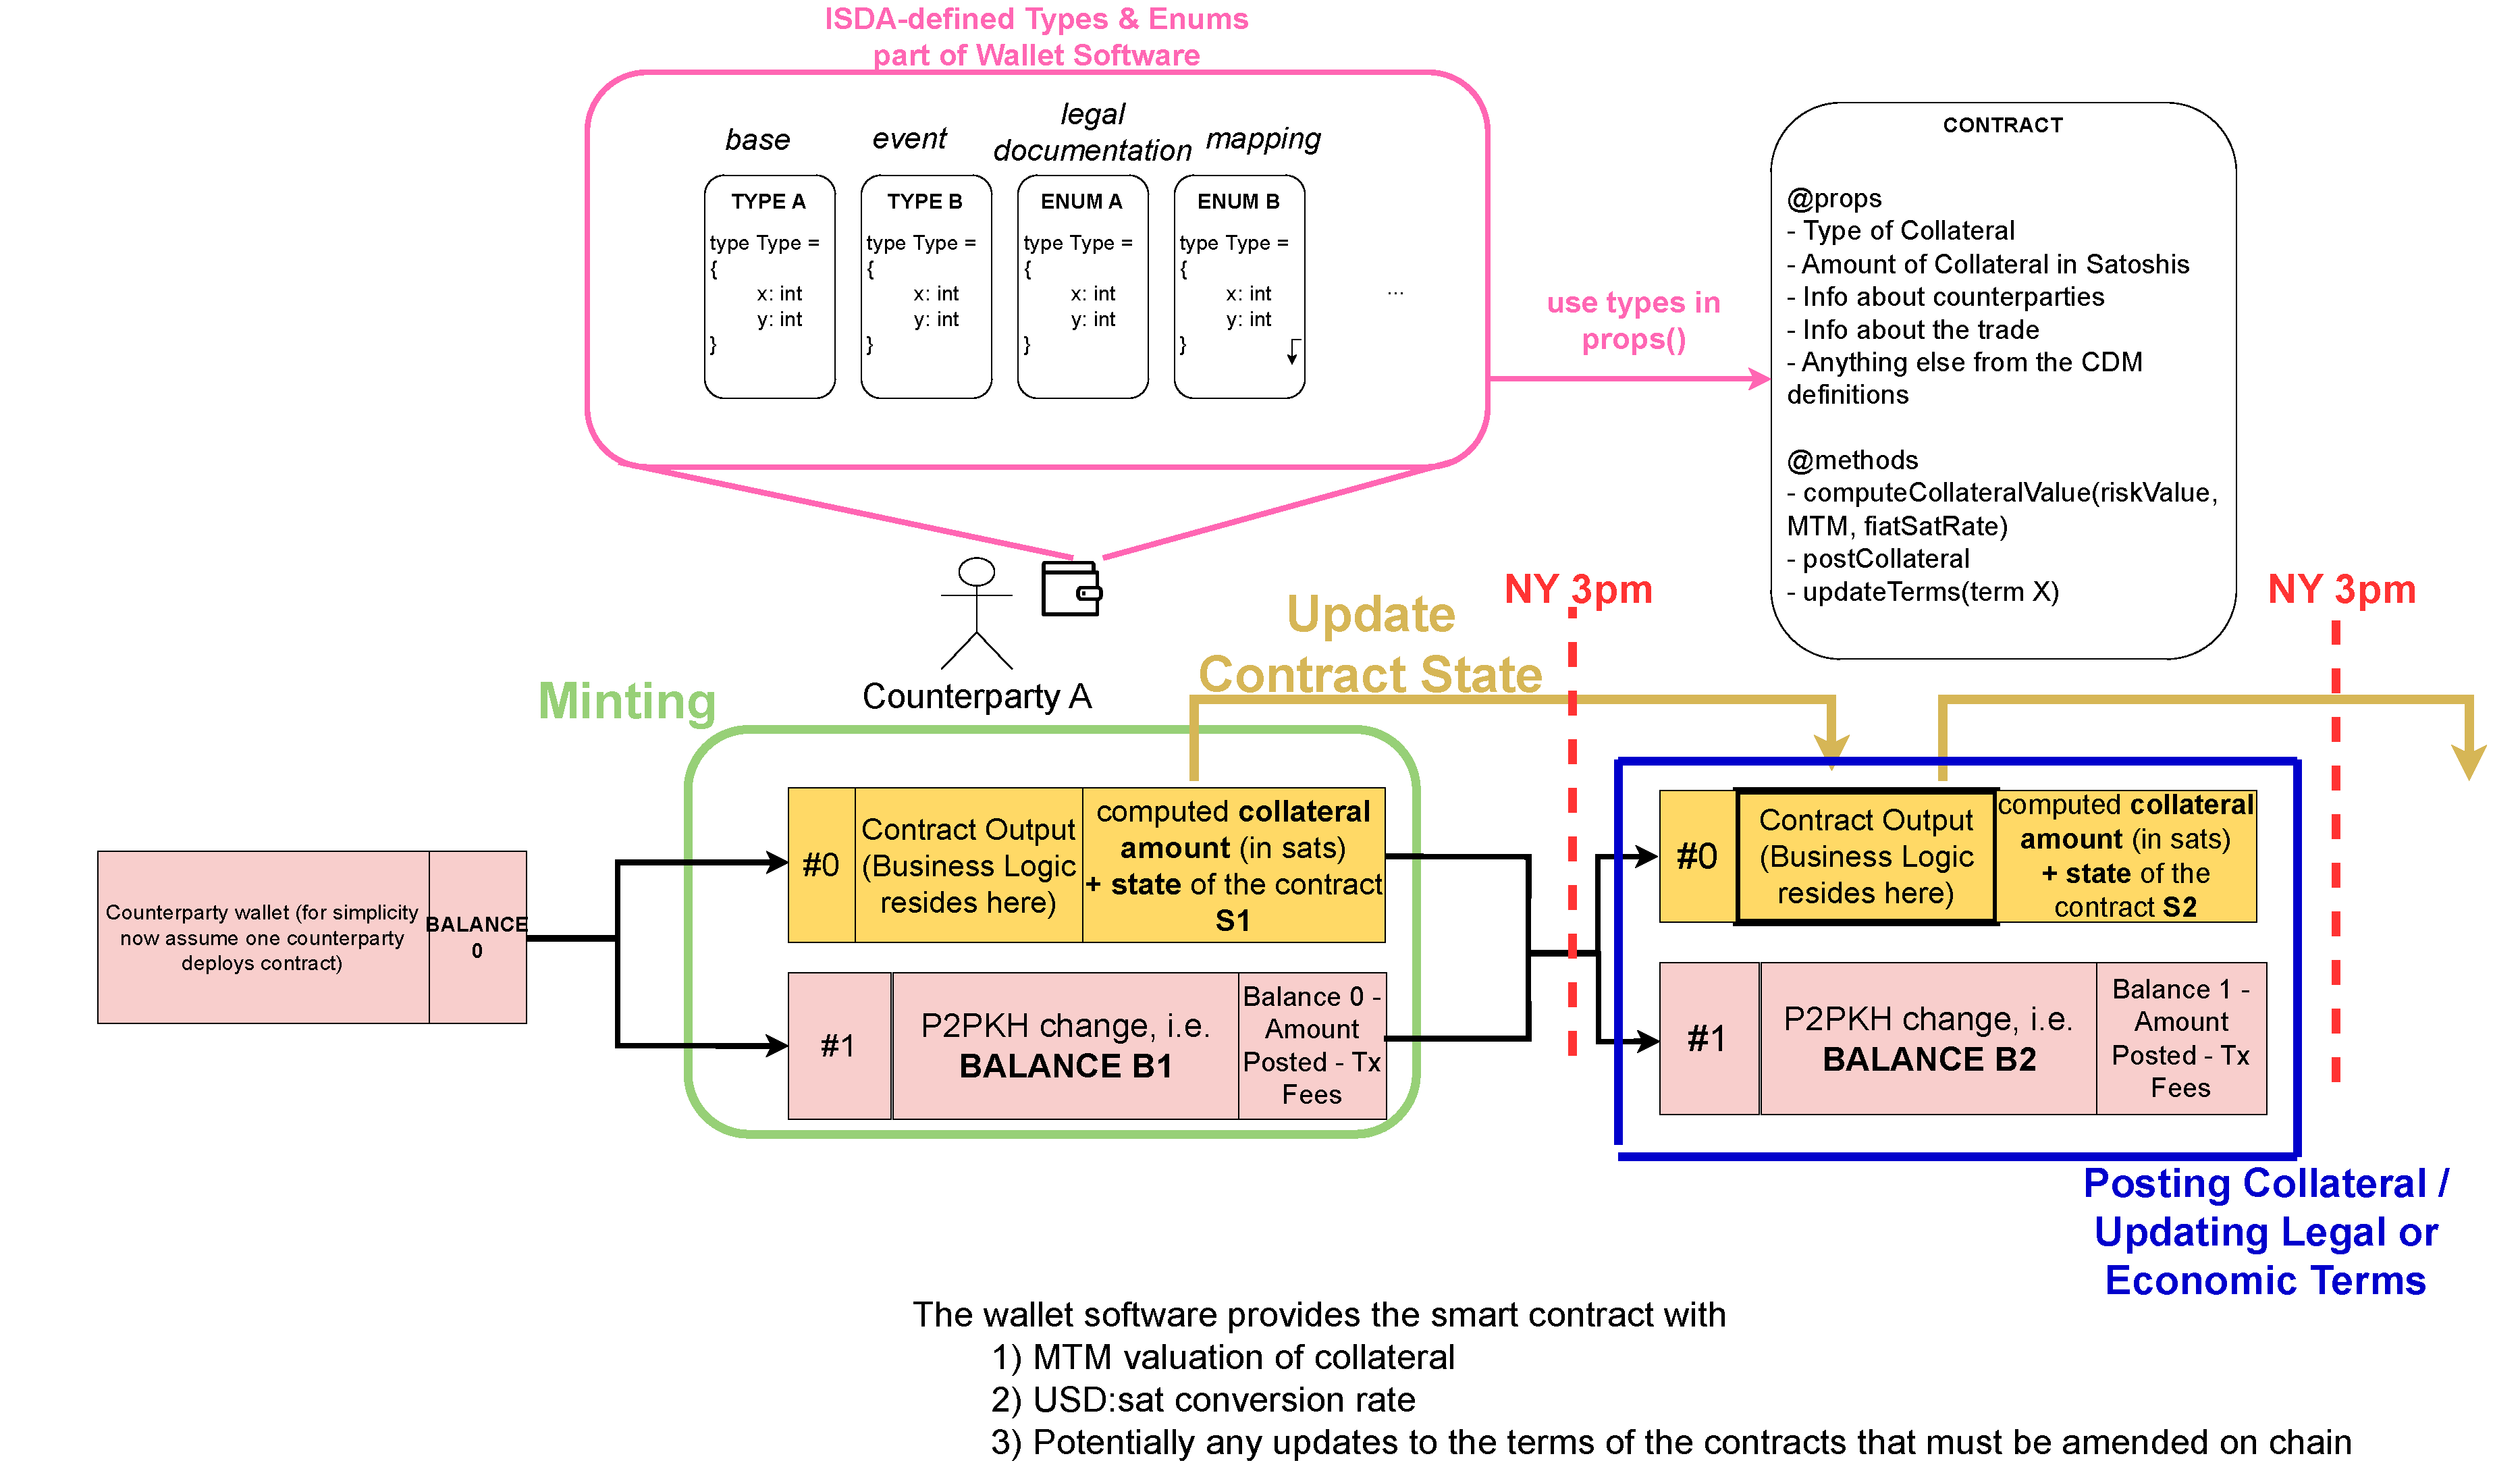
\includegraphics[angle=90, width=0.85\textwidth]{images/chapter 3/Architecture (for draft).drawio.pdf}
    \caption[High-Level Architecture Diagram]{The diagram illustrates the key components of the system. The Wallet software incorporates ISDA Common Domain Model type definitions to populate smart contracts with essential properties. UTXOs are categorized as Smart Contracts (yellow) and Balances (pink). Collateral relationships begin with Minting and can be modified through Collateral Posting or Economic Terms updates. Collateral re-evaluation occurs regularly (e.g., at 3pm New York time) to accommodate potential price fluctuations.}
    \label{fig:architecture-diagram}
\end{figure}
\restoregeometry

As the UTXOs are spent and contract state and balances are updated (details in Section \ref{sec:flow_of_events}), a chain of successive lifecycle states is formed, which together represent the entire collateral relationship between the two parties throughout time. Multiple UTXO chains, and thus series of smart contracts, can exist between the same two counterparties at the same time, each for a specific collateral relationship, and we define each one as a \textit{UTXO Set}. It is important to highlight that the system has checks in place to verify that a piece of collateral pledged in one UTXO Set cannot be utilised in another UTXO Set. By inspecting a UTXO Set, the entire history of the relationship can be inspected and thus audited, easing the job of regulatory compliance. Figure \ref{fig:custodian} shows a visual representation of UTXO Sets where a custodian still plays the role of a middleman between the two counterparties and holds assets on their behalf, thus being responsible for interacting with the chain and creating the UTXO Sets. The relevance of the figure of the custodian in this context is dicussed in further detail in Section \ref{fig:custodian}.

\begin{figure}[!h]
    \centering
    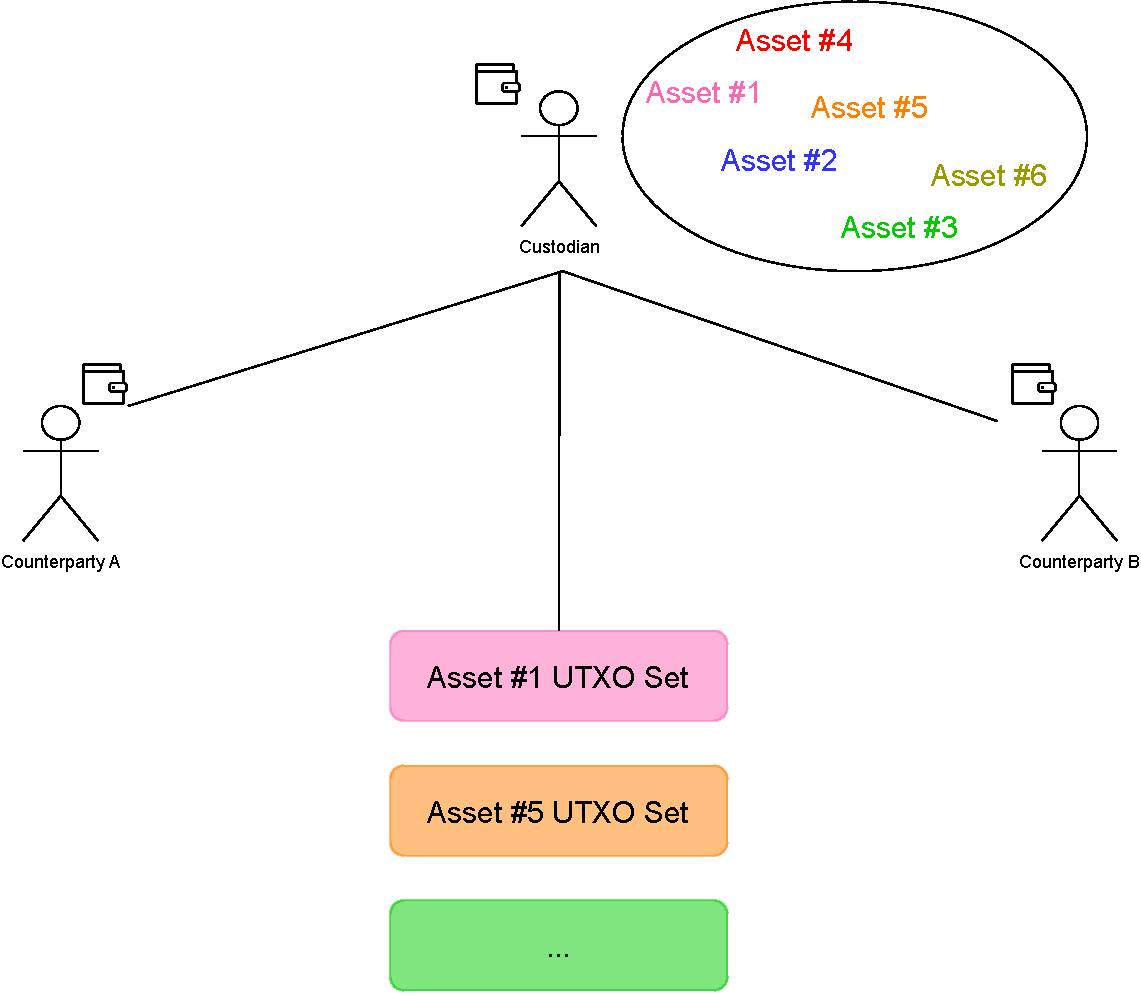
\includegraphics[width=0.5\textwidth]{images/chapter 3/custodian.drawio.pdf}
    \caption[UTXO Sets]{The Custodian wallet manages tokenised assets for counterparties. UTXOs linked to the same collateral are organized in UTXO Sets. An unlimited number of distinct UTXO Sets can exist between the same two counterparties. The diverse colors within the image represent the various assets held by the custodian, all of which can be pledged as part of a single UTXO Set at any given moment. Upon termination of a collateral relationship, the pledged assets become available for use in another UTXO Set.}
    \label{fig:custodian}
\end{figure}




\section{Mapping Common Domain Model to Smart Contracts}
\label{sec:mapping}

A significant amount of time has been spent on designing the conversion from the ISDA Common Domain Model (see Appendix \ref{app:cdm}) to a functionally equivalent representation in Typescript, more specifically in a sCrypt-compliant format. This requirement posed some technical challenges that we will expose in this section. The design principles behind the original Rosetta implementation are described on the official ISDA CDM website \citep{cdm_website}, however a Typescript implementation is also provided \citep{cdm_typescript}. While a good starting point, we note that the Typescript implementation is heavily outdated and does not reflect the latest changes in neither the Typescript language style formats, resulting in numerous compiler errors that had to be manually fixed, nor, more crucially, in the CDM definitions themselves, leading to extensive manual reconciliation work between the two sources. Our suggestion to ISDA, as described in chapter \ref{ch:conclusions}, is to create an automation tool to update the distributions in the different languages the CDM is provided in (including many of the most popular programming languages such as Python, Java, Scala, C\#, Go and Typescript) to reflect the up-to-date changes to a single source of truth. This would require knowing the inner workings of the different languages and is outside the scope of this work \label{cdm_tool}.

The first step consisted in creating a visual representation of the type system defined in the Rosetta Domain-Specific Language originally used to publish the CDM. This can be observed in Figure \ref{fig:mapping}, showing a tree-like structure where nodes represent types and edges represent connections between types, with a directed edge from type A to type B if type A references type B in its definition.

The visual representation allowed us identify three semantically logical groupings between different types which we define as the \textit{Relationship}, the \textit{Portfolio} and the \textit{Position}, each represented as a distinct contract in the final system design.

\begin{itemize}
    \item \textbf{Relationship}. This represents the overarching trading relationship between the counterparties independent of any specific piece of collateral. It includes references to multiple collateral portfolios, provisions for the collateral agreement (such as the type of eligible collateral, the collateral types accepted by the counterparties, or the substitution provisions) and details on the Independent Amount (IM). This serves as an extra cushion of collateral that the counterparty requires to be posted to mitigate the credit risk associated with the other party. This amount is independent of the mark-to-market valuation of the derivative contract \citep{IM}. The most noticeable difference between the original CDM and our solution relates to how the information about the counterparties is represented for the purposes of payments, in this specific context relating to IM but extending beyond that. The CDM utilises two pieces of information, the \textit{Payer/Receiver Account Reference} and the \textit{Payer/Receiver Party Reference} to uniquely identify a counterparty. These have been replaced by the BSV address of the parties' wallets. See Appendix \ref{app:relationship} for the source code of the Relationship contract.

    \item \textbf{Portfolio}. This represents a collection of collateral positions all governed by the same legal agreement. The portfolio contains a list and corresponding identifiers for the individual positions, and it is in turn contained in a Relationship. An aggregate balance is computed by taking into account the valuation of all the individual pieces of collateral. In our solution, this translates to storing and fetching all the UTXOs corresponding to the Positions and summing the amounts of satoshis locked in those UTXOs. See Appendix \ref{app:portfolio} for the source code of the Portfolio contract.

    \item \label{item:other_assets}\textbf{Position}. This represents the specifics of a piece of collateral, including its type, any treatments applied to it such as different types of haircuts\footnote{"Haircuts" refer to the percentage reductions applied to the value of collateral provided by a counterparty to account for potential market fluctuations.}, and the history of movements of that collateral piece (the \textit{Price Quantities} in Figure \ref{fig:mapping}). Two noticeable differences must be pointed out here related to the redundancy of specific attributes. Firstly, the \textit{Settlement Status Attribute}, used to specify whether the valuation associated with the collateral includes amounts that have already been settled, amounts that have not been settled yet or both, is not of much use in a blockchain context where settlement is (close to) immediate. In fact one of the key advantages offered by the system is the immediacy with which trades are settled and reduced reconciliation efforts. We deemed the attribute redundant and decided to exclude it from the final system. Secondly, and relatedly to what has been just described, the \textit{Settlement Terms} attribute connected to specific movements of the collateral becomes redundant and have thus been excluded from the system design. Finally, the CDM allows for different asset types to be represented, as shown by the \textit{Underlying Product} attribute. However, due to time limitations with this dissertation and for the purposes of implementing a viable proof-of-concept, we restricted ourselves to one type of underlying, namely commodities, more specifically crude oil, as mark-to-market valuations would be easier to compute compared to more complex products such as interest rate swaps or indexes. Support for other types of underlyings is suggested as future work in Chapter \ref{ch:conclusions}. See Appendix \ref{app:position} for the source code of the Position contract.
\end{itemize}

\newgeometry{top=1cm}
\thispagestyle{empty}
\begin{figure}[!h]
    \centering
    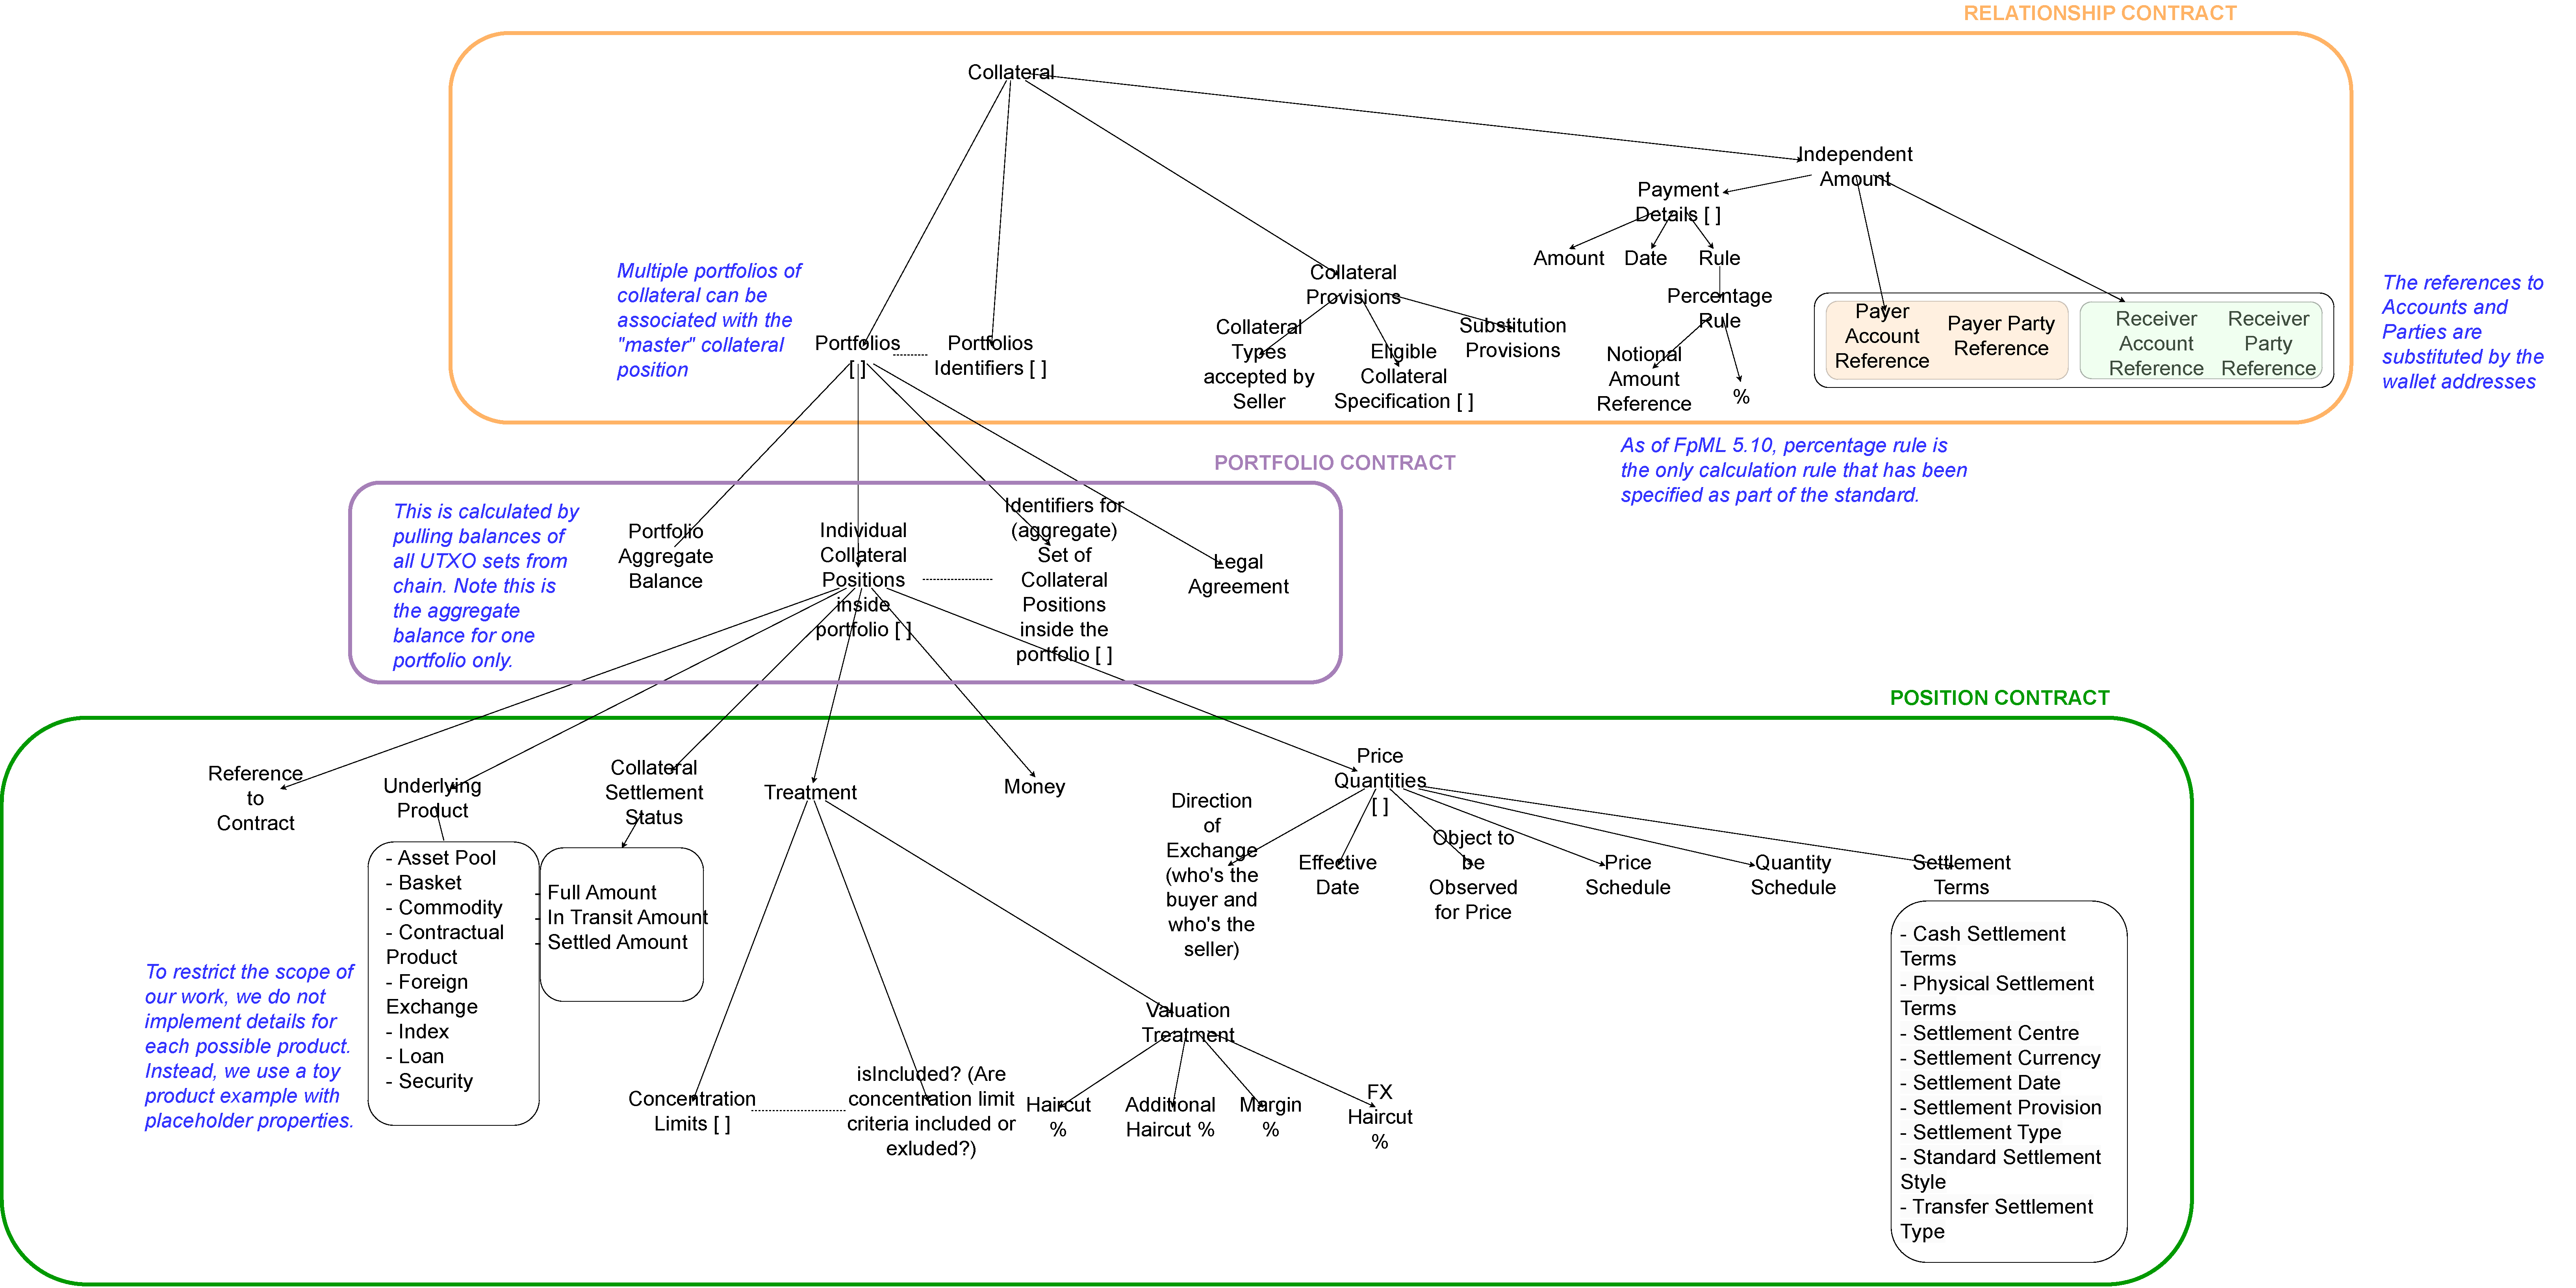
\includegraphics[angle=90, width=0.8\textwidth]{images/chapter 3/mapping (for draft).drawio.pdf}
    \caption[Mapping Common Domain Model to Smart Contracts]{Illustration of the ISDA Common Domain Model (CDM) in a tree-like arrangement. Incoming edges denote containment of one type within another. The CDM is organized into three tiers of smart contracts. The Relationship contract signifies the trading relationship between counterparties, unrelated to specific collateral. The Portfolio contract oversees a group of collateral positions under a shared legal agreement. The Position contract outlines collateral details like type, treatments, and history of movements. }
    \label{fig:mapping}
\end{figure}
\restoregeometry

A key aspect of the dynamics between the different contracts is the ability to reference each other in multiple directions (e.g. fetching individual collateral positions starting from the relationship as well as retrieving the relationship details from any one position). Two approaches have been considered to include this property in our system.

\begin{enumerate}
    \item \label{item:arrays} Our original approach envisioned using arrays to store references to other contracts in the form of UTXO addresses. A challenge was quickly encountered in this scenario due to the fact that sCrypt's array implementations does not allow for variable-sized arrays, only fixed-size \citep{scrypt_arrays}. This would make it impossible to append new portfolios to a relationship or positions to a portfolio. As a workaround to this issue we originally considered storing only references from 'children' contracts to 'parents', removing the \textit{Individual Collateral Position Portfolio} array from a Portfolio and the \textit{Portfolios} array from a Relationship. This way, deploying a new Position, for example, would only require knowing the address of the containing Portfolio at deployment time and include it in the Position, and no arrays would have to be modified. Implementing the bi-directional retrieval capability would have required, however, some complex reverse-indexing \citep{inverted_index} taking place off-chain. This solution appeared cumbersome and complex and was therefore discarded.

    \item We developed an alternative solution, which is the one currently adopted by the system, after support talks with the main sCrypt developers. This solution uses HashedSet to store references to UTXO addresses. An HashedSet \citep{hashed_set} is defined as a special type of HashedMap \citep{hashed_map}, a data structure that efficiently stores key-value pairs by using a hash function to compute indexes for quick retrieval and insertion. A HashedSet is a subtype of a HashedMap where values are identical to their corresponding keys and are thus omitted. A key aspect of the sCrypt implementation of HashedSets is that only the hash values of the keys are saved on the chain, meaning that off-chain copies of the items in the set must be stored locally to be able to deserialize the set into an intelligible representation (hash functions are designed to be one-way functions, making it extremely difficult to retrieve the original input from the hash value \citep{invert_hash_functions}). While adding some technical complexity to the final solution, this approach achieves the bi-directional referencing currently supported by the CDM and we deemed this design to be more feasible and elegant than the original one involving arrays

\end{enumerate}

As already mentioned, mapping the CDM to sCrypt has proven particularly challenging for a number of technical reasons described below:

\begin{itemize}

    \item \textbf{Data types supported by sCrypt}. sCrypt supports three main basic data types, namely \textit{boolean}, \textit{bigint} and and \textit{ByteString}. While the CDM also uses the boolean type, it relies on the \textit{number} and \textit{string} primitives. All references to these two data types had to be converted to \textit{bigint} and \textit{ByeString}, respectively. The rationale behind the choice of these two particular data types to represent numbers and text is not provided in the sCrypt documentation, and while requiring some manual work to convert the CDM, we speculate on the utility of these two data types specifically in a blockchain context:

    \begin{itemize}
        \item \textbf{Bigint} (represents numeric values which are too large to be represented by the number primitive in Typescript \citep{bigint}).
        
        \begin{itemize}
            \item \textbf{Precision}. BSV operates on very large numbers, especially when dealing with satoshis. Regular \textit{numbers} have limited precision, while \textit{BigInt}s can accurately represent and perform arithmetic operations on integers of arbitrary size without loss of precision (and only a 5.30\% performance difference as measured in arithmetic operations per second at the time of writing \citep{bigint_number_performance}).
            \item \textbf{Consistency with Bitcoin Protocol}. The Bitcoin protocol itself uses 64-bit integers for various purposes, therefore BigInt is a better match for representing these integers in a way that aligns with the underlying protocol.
            \item \textbf{Security and Trust}. Using BigInt helps minimize the risk of bugs caused by floating-point inaccuracies and ensures that the code behaves as expected.
        \end{itemize}
        
        \item \textbf{ByteString} (represents arbitrary binary data, ensuring this is handled as raw bytes rather than interpreted characters)

        \begin{itemize}
            \item \textbf{Script operations}. BSV transactions often involve manipulating raw binary data (like public keys, hashes, signatures) rather than traditional text data. Using ByteString can help represent this data more accurately and efficiently.

            \item \textbf{Hexadecimal Representation}. in BSV data is often represented in hexadecimal format (base16). Using a ByteString or binary data representation can make it easier to work with and manipulate these hex-encoded values.

            \item \textbf{Data (De)serialization}. Data serialization and deserialization efficiency\footnote{Efficiency here encompasses both temporal and spatial considerations. Compact data representations are crucial because blockchain memory is a limited resource; using it judiciously minimizes transaction fees. Additionally, quick data operations are imperative for supporting the high throughput of transactions in the financial derivative contexts.} is pivotal due to constraints such as block size limitations. Binary data representation can facilitate more compact serialization formats, thereby optimizing both transaction size and associated fees.

            \item \textbf{Data Integrity}. Using binary data representation can help ensure data integrity by preventing unintended character encoding or transformations that could affect calculations.
            
        \end{itemize}
        
    \end{itemize}

    \item \textbf{Floating point numbers}. While the BigInt datatype ensures higher precision with integer calculations, it does not support floating point calculation, which in our context would be required. For example, the spot price of an asset or the exchange rate between USDC and BSV are all floating point numbers. The current solution truncates the decimal part by taking the floor of the floating point number. Possible workarounds to this barrier are discussed in Section \ref{ch:conclusions}.

    \item \textbf{Dates}. The CDM relies on the built-in Date object in Typescript to represent points in time \citep{dates}. Consistency with this approach would have required translating part of the Typescript implementation itself to utilise the basic sCrypt data types, which we considered out of the scope for this work. A suggested workaround is to simply use a BigInt value that represents the UNIX epoch time (the number of milliseconds since the midnight at the beginning of January 1, 1970, UTC \citep{epoch})

    \item \label{item:generics} \textbf{Generics}. These are reusable and flexible code components in Typescript that allow types to be parameterised, enabling functions, classes, and interfaces to work with different data types while maintaining type safety and preventing the need for code duplication \citep{generics}. For example, the \textit{FieldWithMeta$\langle $T $\rangle$} interface defined in the \textit{metatypes.ts} file of the CDM allows to encapsulate a value of any generic type $T$ along with accompanying metadata within a single structure. Generics are not supported by sCrypt, the compiler yielding an \textit{Invalid Type} error. A possible workaround to to this obstacle would be to create specific variations of the generic interface for all possible types to be supported (sCrypt does support user-defined types \citep{user-defined-types}), effectively violating the very purpose of generics. This has not implemented in the current version of the system as it would have required significant additional manual work that would have not added any major benefits for the purpose of the proof-of-concept and is suggested as future work.

    \item \textbf{Arrays}. As already mentioned on page \pageref{item:arrays}, sCrypt only supports fixed-size arrays. This poses an issue when a type contains arrays that could potentially be empty at deployment and will need to be filled in later. For example, the \textit{EligibleCollateralCriteria} interface contains an array of \textit{IssuerCriteria[]}, specifying requirements or qualifications that an issuer of a financial instrument must meet in order for that instrument to be considered acceptable as collateral, which could be potentially empty at the beginning in case no criteria apply to the type of issuer of the instrument. Assuming the arrays are fixed-size, it makes sense that the compiler would not allow to use empty arrays as these could not be modified while at the same time occupying block size. We originally tried to apply the same workaround described on page \pageref{item:arrays} utilising \textit{HashedSet}s instead of arrays, however the compiler would still throw errors in case the HashedSet was empty at deployment. A possible solution --- not implemented in the system, which currently simply ignores empty arrays --- would be to redeploy a new contract when the values to populate the array are known, ignoring the UTXO corresponding to the previous state.

    \item \label{item:circular_deps} \textbf{Circular dependencies}. In a strongly typed language like TypeScript, a circular dependency between types occurs when two or more types depend on each other directly or indirectly. This can lead to a situation where the types reference each other in a way that creates a loop, making it difficult for the compiler to properly infer and resolve the types \citep{circular_dependencies}. In the CDM, many circular dependencies are present. For example, the \textit{Underlying Product} for the collateral position could be of type \textit{Basket}, which contains multiple \textit{Basket Component}s that could potentially be \textit{Basket}s themselves. Such dependencies would prevent compilation from succeeding, therefore we had to manually amend the types that were generating the problem. While far from optimal, we opted for this workaround as a more thorough solution would have required a deeper overhaul of the CDM itself which was outside the scope of this work. As discussed in \ref{ch:conclusions}, we suggest close collaboration between sCrypt developers and CDM should be fostered to increase the level of interoperability between the two tools.

    
\end{itemize}
\section{Flow of Events}
\label{sec:flow_of_events}

The lifecycle of a piece of collateral, and its UTXO Set on-chain, can be broadly split into two stages (refer to Figure \ref{fig:architecture-diagram}):

\begin{enumerate}
    \item \textbf{Minting}. This is the initiation of the UTXO set. The Wallet software creates the smart contract by using the CDM type system, and consumes an existing UTXO representing the balance of the party minting the collateral to create two new UTXOs: the contract and the remaining balance.  
    \item \textbf{Posting/Updates}. At regular time intervals the state of the UTXO Set is updated to reflect changes in collateral valuation (note that this functionality is not currently implemented but could easily be achieved by running a \textit{"cron job"} \footnote{A "cron job" process is a scheduled task or automated script in Unix-like operating systems that runs at specified intervals without the need for manual initiation \citep{cronjobs}.} process in the background). The updating transactions consumes two inputs, the current contract state and balance of the counterparty, and produces two new UTXOs: the updated contract state (potentially containing a different amount of satoshis) and the updated balance. These updates can be of two types:
    
    \begin{enumerate}
        \item \textbf{Posting/Receiving Collateral}. This type of update refers to movement of satoshi to either the contract or the party's balance depending of the new valuation.
        
        \item \textbf{Updating Contract Terms}. this type of update allows the custodian to modify the business logic of the contract (e.g. the eligibility of an existing or new type of collateral could be updated). Recounting that legal and economic terms from both the ISDA Master Agreement and the CSAs can be updated in the current sysytem, supporting this functionality is core to a smooth transition the on-chain solution.
    \end{enumerate}
    
    In the current implementation 3pm New York Time (ET) has been arbitrarily chosen as the time to update the UTXO Set, however this level of granularity is quite rough and would not account for intra-day valuation variations. An additional piece of functionality that constantly monitors the state of the market and the valuation of the collateral and updates the UTXO Set whenever a specified threshold valuation is passed would be a good solution to reflect large swings in the market. This is suggested as future work on the this thesis. \label{ny3pm}
\end{enumerate}

A more granular view of the flow of events is provided in Figure \ref{fig:sequence-diagram}, where a sequence diagram of the system is described. The two sections of the sequence diagram correspond to the Minting and Updating stages described above.

\begin{enumerate}
    \item \textbf{Minting}. Let us assume that a custodian is in charge of interacting with the chain. The act of minting requires three smart contracts to be written, the Relationship, the Portfolio and the Position (details on the contents of each are described in more detail in Section \ref{sec:mapping}). The custodian will first deploy the Relationship contract. Only after this has been deployed on-chain can the custodian include the address of its UTXO in the Portfolio contract and deploy the latter. A key aspect of mechanism of the current system is that all objects (within the collateral context as well as beyond it) contain references to each other, and such interconnectedness allows for easy retrieval and inspection beginning with any starting point (one could go back to the trading relationship between parties from a specific collateral position or vice versa, fetch all the positions contained within a relationship). Adapting this mechanism on-chain involves reflecting any change to a '\textit{sub-contract}' (hereby defined as a contract referenced by another one) by updating the \textit{'parent'} contract(s) (the referencing contracts). In the Minting scenario just described, the fact that the Portfolio contract has been deployed must be propagated upwards to the corresponding Relationship within which the Portfolio is contained. In a similar manner, when the Portfolio has been deployed, the Position contracted can be filled in with the Portfolio UTXO's address, published on chain and the deployment information (which takes the form of a UTXO address itself) propagated up the stack to the Portfolio and the Relationship. \label{minting}
    
    \item \textbf{Updating}. The type of update described here corresponds to the movements of satoshis following a change in collateral valuation. Updates of the legal and/or economic terms have not been implemented as the core value proposition of this work is to streamline the valuation and margin-posting elements. While contract term updates would be a required feature of a fully CDM-compliant system, we leave this implementation as future work. Margin calculation and posting follow the steps desribed below:

    \begin{enumerate}
    
        \item \label{item:legal_econ_terms} The Wallet must compute the Mark-to-Market (MTM) valuation for the asset. Depending on specific type of asset, the MTM calculation may vary (e.g. for commodities this is simply the spot price multiplied by the quantity of the asset held as collateral, while for interest rate swaps more detailed calculations involving the fixed and floating rates, as well as the market rates for the corresponding fixed and floating rates, are required). For the purpose of a proof-of-concept, this thesis uses a commodity, crude oil, as collateral. Note that the system is easily extendable to support other types of commodities simply by plugging in the MTM valuation models that a counterparty may already use. The commodity spot price is fetched from the party's preferred traditional financial API, e.g. the Bloomberg terminal. This work used the free and open-source Yahoo Finance library \citep{yfinance, yfinance_python} (see Appendix \ref{app:oracles_yfinance}. In the initial version of the system we planned to use an oracle to provide the spot price and/or MTM, since relying on a traditional API introduces the risk of valuation mismatches should the parties use different sources for their calculations. We were unable to find public oracles providing the service and we attribute this to the low level of maturity of the technical ecosystem, however adapting to changes in 3rd party services provided in this context is suggested as a direction of future work.

        \item \label{item:valuation} The valuation of the collateral should be expressed in satoshis in order to facilitate the movement of collateral. Denominating the asset in satoshis require converting the preferred fiat currency of the parties to satoshis, and this could be accomplished by fetching the exchange rate from an oracle service. In this thesis we use the WitnessOnChain oracle service \citep{woc_oracle} to fetch the exchange rate between USDC and BSV (see Appendix \ref{app:oracles_yfinance}. USDC is a stablecoin, i.e. a digital token whose value is pegged to USD, in the case of USDC specifically via reserve-based pegging. Each USDC is redeemable for one dollar, and is backed by one dollar or a dollar-denominated asset with equivalent value held in accounts at regulated U.S. financial institutions. Those accounts are audited by U.S. accounting firm Grant Thornton LLP, which issues monthly attestations on the reserves backing USDC \citep{pegging_usdc}. While we initially wanted to convert from USD to BSV (as USD is the currency most widely adopted in current collateral relationships), we were not able to find an oracle service providing this specific conversion rate. While relying on USDC is not optimal, the system can be considered safe as long as the stablecoin maintains its peg. An extra layer of security to protect against the fluctuations in the USDC-BSV exchange rate would be to apply an additional haircut to the CSA of the collateral agreement, effectively treating the conversion as a traditional foreign exchange rate. A haircut is a reduction applied to the value of an asset expressed as a percentage of its value \citep{haircut}. For example, if the average fluctuation of the USDC-BSV exchange rate over the previous week was 5\%, a 5\% discount haircut could be applied to the collateral. The full implications and implementation of this solution are left as future work on this dissertation.

        \item The Wallet then fetches the current collateral value stored in the Position contract. This is required to determine whether the collateral has increased or decreased in value.

        \item \label{item:risk_calc}The Wallet then computes the new value of the collateral by using the MTM valuation and the USDC-BSV exchange rate. Note that at this stage any additional factors traditionally used in asset valuation, e.g. specific risk models such as Value-at-Risk (VaR) \citep{VaR}, SPAN (Standard Portfolio Analysis of Risk) \citep{SPAN} or custom Monte Carlo Simulations \citep{monte_carlo}, can be incorporated. Performing these calculations off-chain introduces an additional risk factor since a counterparty must trust the results that the other party provides, fundamentally nullifying one of the core value propositions of this thesis, i.e. the transparency of the margin calculations. An ideal solution would work entirely on-chain, with the calculations, or at least the parameters used in them, publicly auditable. While outside the scope of this work, a thorough analysis of the theoretical and technical aspects of implementing risk calculations at least partly on-chain represents an essential component in fully delivering the benefits that a transition to blockchain purports to offer. Details on how this solution could potentially look like are provided in the Suggestions for Future Work \ref{ch:conclusions}.

        \item The Wallet then updates the Position contract to reflect the newly computed collateral valuation. This information is stored in a property of the smart contract so that it can later be used to verify whether the difference in valuations computed in the successive steps is correct.

        \item The Wallet computes the difference in satoshis between the previous and current valuations of the collateral.

        \item Depending on whether the valuation has risen or dropped, an amount of satoshis corresponding to the difference is transferred to either a P2PKH balance UTXO for the counterparty, in the former case, or to a new contract UTXO in the latter (see Appendix \ref{app:updating_collateral}). Note that whenever UTXOs are spent or updated, changes must be propagated to all referencing contracts (as described in \ref{minting}), hence the \textit{updatePortfolio} and \textit{updateRelationship} functions that appear in the sequence diagram.
        
    \end{enumerate}
    
\end{enumerate}
\thispagestyle{empty}

\newgeometry{top=1cm}
\begin{figure}
    \centering
    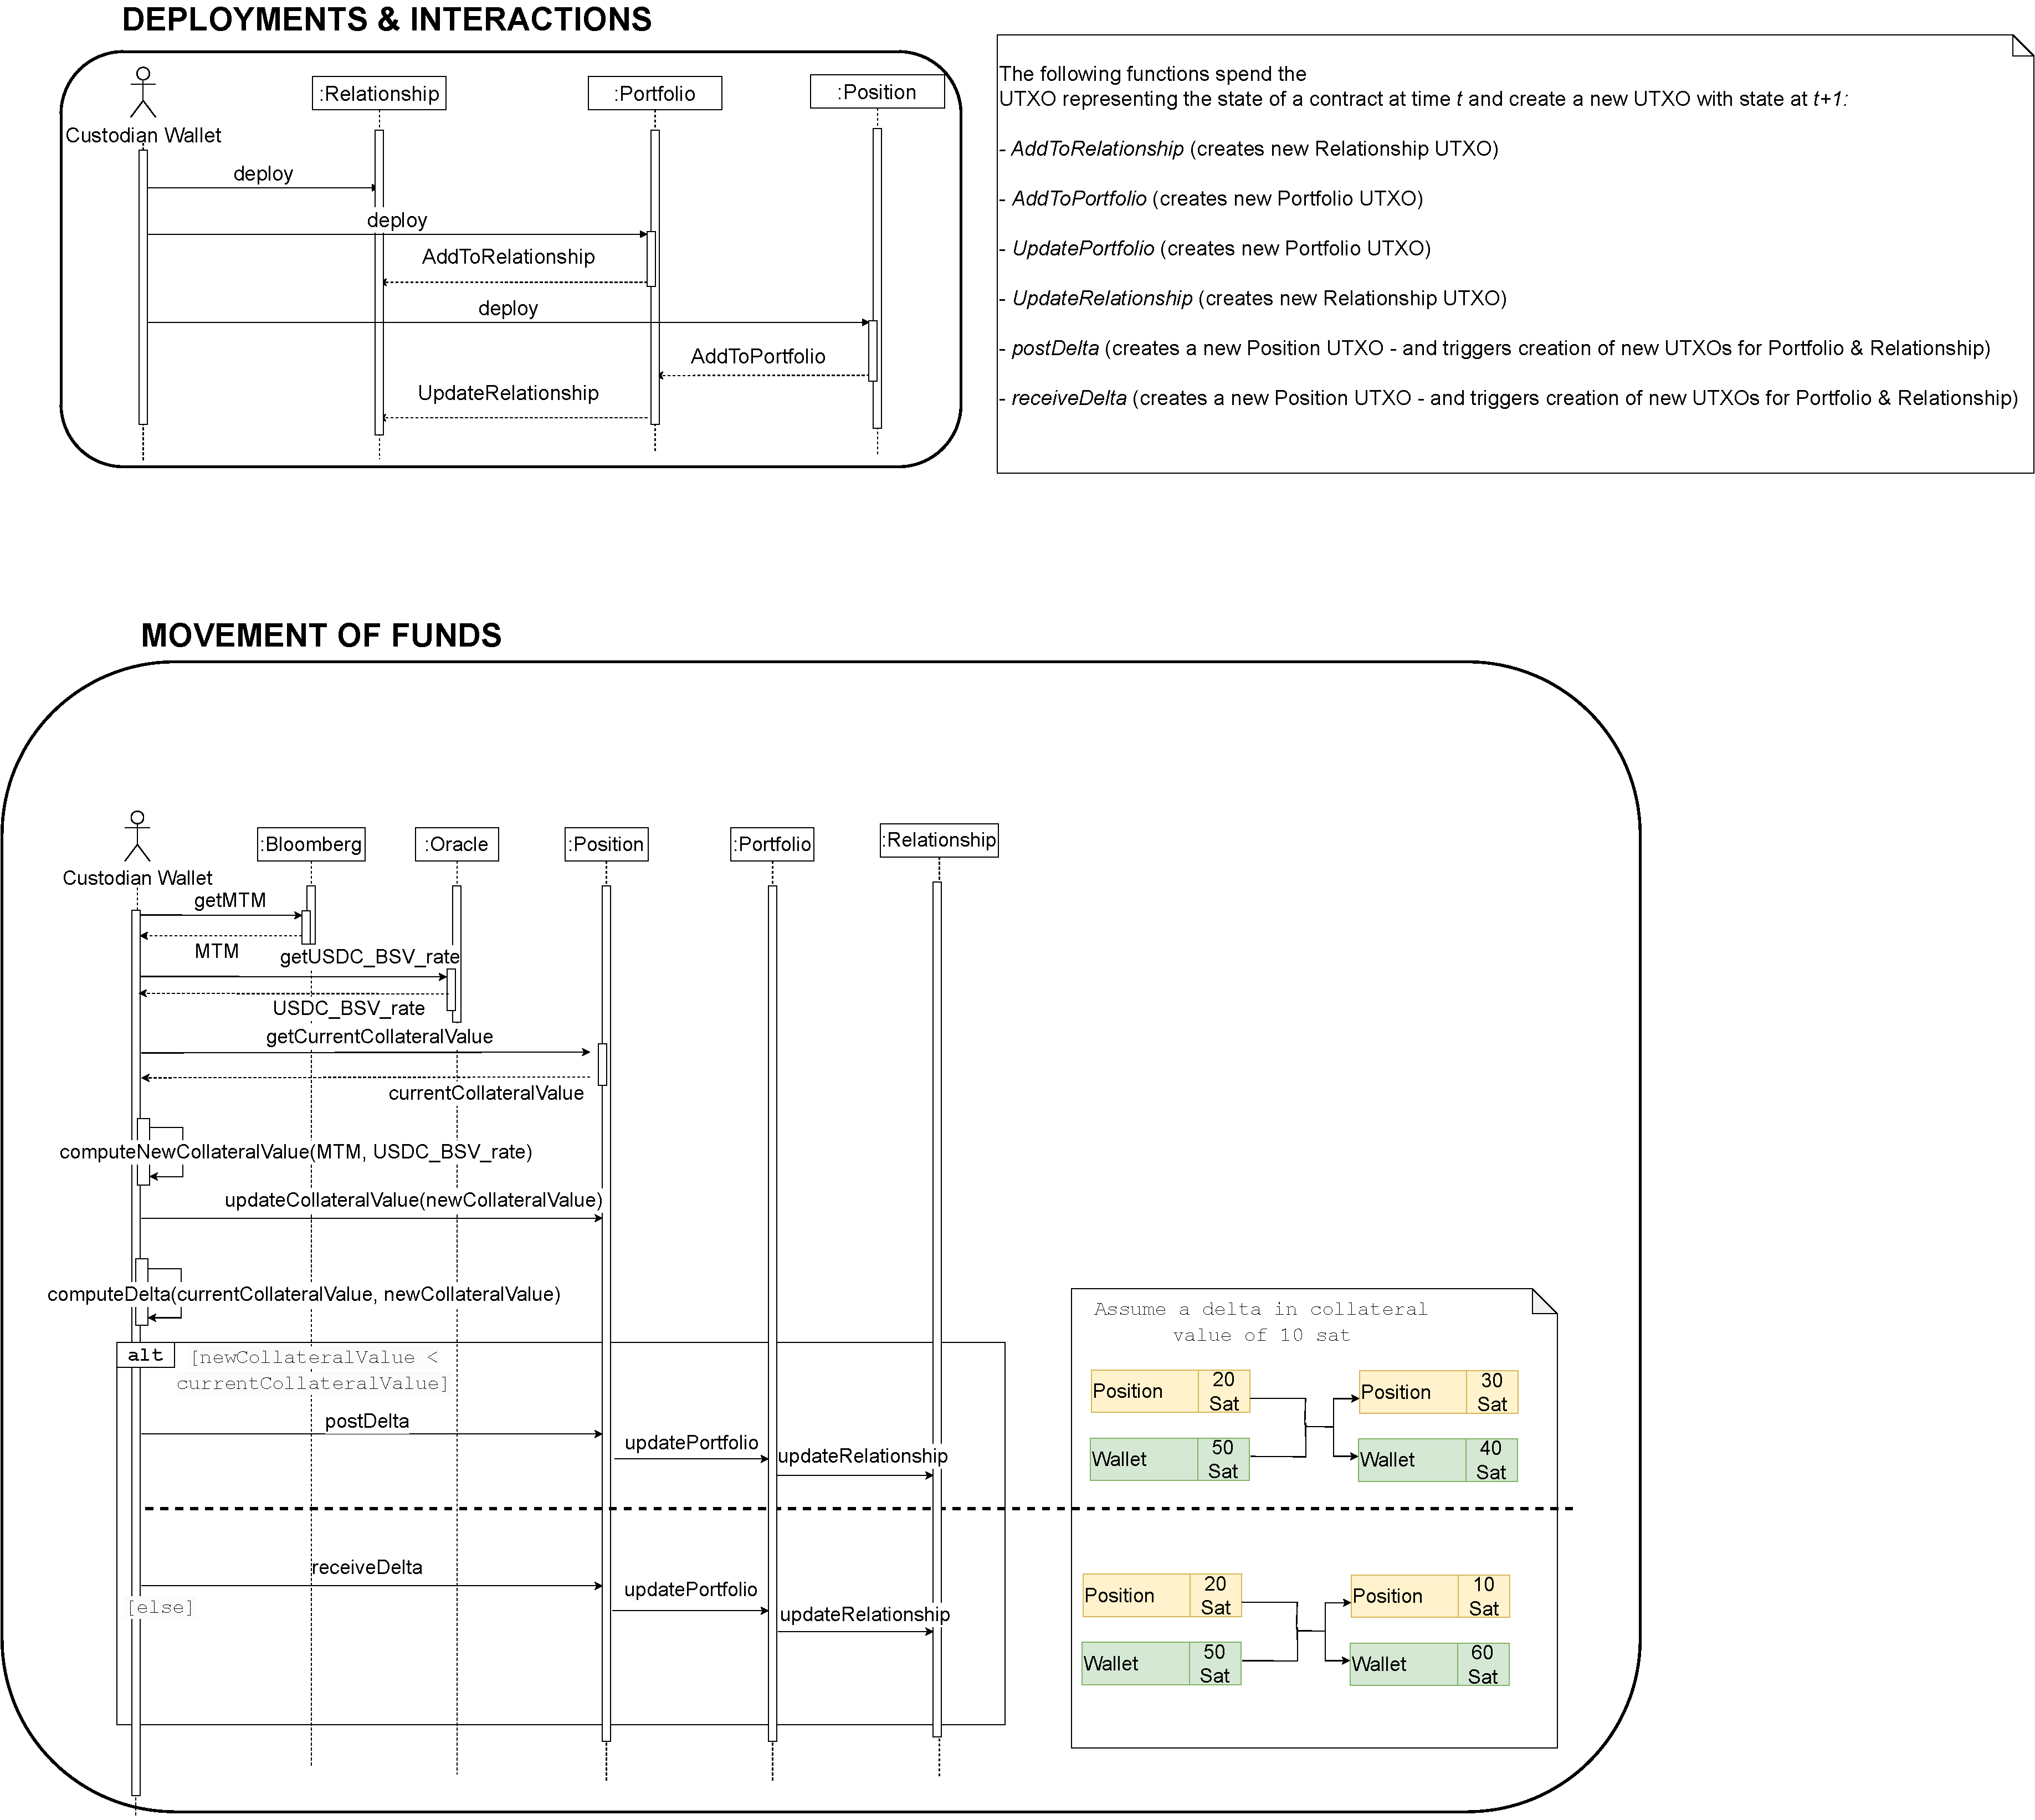
\includegraphics[angle=90, height=\textheight, width=\textwidth]{images/chapter 3/sequenceDiagram.drawio.pdf}
    \caption[Sequence Diagram]{Sequence diagrams depicting the steps in the collateral smart contract lifecycle. The upper diagram displays the initial deployment of three smart contracts: Relationship, Portfolio, and Position. The lower diagram illustrates the process of reassessing collateral value due to market shifts, incorporating data from oracles and financial APIs. It also showcases the adjustment of satoshi amounts to align with collateral valuation changes.}
    \label{fig:sequence-diagram}
\end{figure}
\restoregeometry


% ################ CHAPTER 4 ################ 
\chapter{Results and Discussion}
\label{ch:resultsDiscussion}
This chapter offers an in-depth analysis of the outcomes associated with the proposed system for tokenizing collateral in derivative trading on the BSV blockchain. Firstly, we discuss how the custodian's role is transformed but still critical (Section \ref{sec:custodian}). We highlight the benefits of a hybrid model that combines automation through smart contracts with human oversight for tasks like risk assessment and compliance. Secondly, we examine the advantages across four domains: financial, economic, legal, and technological (Section \ref{sec:benefits}). This includes discussions on operational cost savings, enhanced market liquidity, regulatory compliance, and how BSV's capabilities align with the system's requirements. Finally, we address the legal aspects of tokenizing collateral, classifying our system as a hybrid model (Section \ref{sec:legal_considerations}). This section highlights how the system manages to meet regulatory requirements while also enabling direct interactions through smart contracts.

\section{On the Role of the Custodian}
\label{sec:custodian}
The role of custodians in our proposed system architecture remains integral but is substantially altered. While functions like record-keeping could be automated via the blockchain's immutable ledger, responsibilities such as risk assessment and compliance assurance still warrant human expertise. The blockchain's capacity for automating record-keeping may reduce operational costs and minimize manual errors, enhancing the efficiency of audits \citep{DTCC}. However, the custodian's role continues to be important in functions like dynamic risk assessments, which necessitate human judgment.

In terms of compliance, smart contracts may automate certain regulatory requirements but fall short in addressing the complexities of varying international laws or rapid legal changes. Thus, custodians act as a safeguard in ensuring all-encompassing regulatory adherence \citep{Thomson_Reuters}.

A new paradigm in custodianship may arise in this setting, characterized by a blend of automation and human oversight. While smart contracts could facilitate instantaneous asset transfers, custodians would retain a role in supervising the initiation and completion of transactions, particularly for handling exceptions or contingencies \citep{isda_transparency}.

This hybrid model of custodianship offers the best of both worlds: it couples the reliability of automated processes with the expertise of human oversight. For instance, a study from the conventional financial sector found that incorporating automated processes along with human supervision decreased transactional errors by nearly 30\% \citep{accenture}. In this context, smart contracts would handle routine operations like immediate post-trade collateral transfers, freeing custodians to concentrate on complex tasks such as liquidity evaluation and risk management \citep{deloitte_costs}. Consequently, this combination streamlines the initiation and settlement processes without compromising on the informed decisions that custodians contribute, resulting in a more efficient and secure trading infrastructure.

\section{Benefits of Solution}
\label{sec:benefits}
 The benefits of implementing the proposed collateral management system are described in this section. We examine the advantages across four key dimensions: financial (Section \ref{subsec:benefits_financial}), economic (Section \ref{subsec:benefits_economic}), legal (Section \ref{subsec:benefits_legal}), and technological (Section \ref{subsec:benefits_technological}). From significant reductions in operational costs to improvements in market liquidity and efficiency, we outline how the solution aims to address existing challenges. We also explore risk mitigation strategies and how blockchain technology can aid in regulatory compliance and dispute resolution. Moreover, the chapter discusses the technological attributes that make the BSV blockchain a suitable choice for this application.
\subsection{Financial}
\label{subsec:benefits_financial}

\begin{itemize}
    \item \textbf{Reduction in operational overheads}. The operational overheads and costs associated with derivatives trading in the realm of collateral management can be substantial. The financial services sector could save more than €4 billion annually in collateral management costs by addressing operational inefficiencies \citep{accenture}. These costs stem from the need for specialized software, manpower, and compliance measures to manage the complex collateral requirements associated with derivatives contracts. Additionally, the advent of regulations like Dodd-Frank in the U.S. \citep{dodd-frank} and EMIR \citep{EMIR} in Europe has led to increased reporting and margin requirements, further escalating costs \citep{costs_doddfrank_emir}. Firms also incur opportunity costs by tying up capital as collateral that could otherwise be invested. A report by Deloitte estimates that collateral requirements could tie up as much as \$1.9 trillion in high-quality assets \citep{deloitte_costs}. Therefore, the operational overheads in collateral management are not just a cost center but also a strategic concern that impacts liquidity and capital efficiency. Our solution promises to relieve trading entities of the operational overheads by proposing a standardized format to tokenize collateral and automating the movement of assets.


    \item \textbf{Enhanced liquidity}. Enhanced liquidity in derivatives trading, particularly through the ease of trading and transferring assets, has a profound impact on the market. By making previously illiquid assets more accessible, the market experiences a boost in trading volume and efficiency. For instance, the securitization of illiquid assets like mortgages or loans into tradable derivatives allows a broader range of investors to participate in markets that were previously inaccessible. According to statistics reported by the Bank for International Settlements (BIS), the global derivatives market has grown to an estimated \$640 trillion in notional amount outstanding, partly fueled by the increased liquidity of assets \citep{bis_costs}. The advent of digital assets has further augmented this trend. Cryptocurrencies and tokenized assets, being easily tradable on various digital platforms, have introduced a new layer of liquidity. They have enabled even more participants to engage in the market, making assets like real estate or art, once considered highly illiquid, more accessible through tokenization \citep{digital_asset_tokenization}. This enhanced liquidity not only fosters market stability by allowing for more seamless price discovery but also promotes economic growth by facilitating capital allocation. Furthermore, it reduces the cost of capital for issuers and provides investors with diversified investment opportunities.

    While the benefits of enhanced liquidity through asset tokenization and digital trading platforms are significant, it's crucial to consider the complexities involved. For instance, the mere act of making a traditionally illiquid asset more tradable does not automatically translate to increased market liquidity. The Central Limit Order Book (CLOB) systems, commonly used in asset trading, may not be well-suited for illiquid assets, as Market Makers often require a wide spread to mitigate the risks associated with the asset's volatility \citep{maureen2001overview}. To address these challenges, we propose two alternative approaches to consider. One such strategy is to restrict the trading window for illiquid assets, thereby concentrating market activity and potentially stabilizing prices. Another approach could be the adoption of Automated Market Maker (AMM) systems, a concept borrowed from decentralized finance (DeFi). AMMs operate on a liquidity pool model where participants deposit assets into a smart contract. These pools can then facilitate trades directly between buyers and sellers without the need for a traditional Market Maker. In the context of illiquid assets, an AMM system allows participants to provide liquidity directly, making the market more robust and efficient \citep{aoyagi2020liquidity}. These nuanced strategies aim to foster a more stable and liquid market, facilitating better price discovery and capital allocation.
\end{itemize}
\subsection{Economic}
\label{subsec:benefits_economic}

\begin{itemize}
    \item \textbf{Increased market efficiency}. Traditionally, the settlement of trades often operates on a "T+2" basis, meaning that the transaction is finalized two business days after the trade is executed. This delay introduces a range of inefficiencies and risks, including counterparty risk and the need for more extensive collateral management \citep{t_2_settlements}. Our solution promises to revolutionize this paradigm by enabling "T+0" settlements—same-day settlement of collateral operations. The acceleration to "T+0" is not merely a technological feat but a transformative shift towards increased market efficiency. According to a report by McKinsey \citep{mckisney_tokenization}, shorter settlement times generate significant savings in high-interest-rate environments such as at the time of writing \citep{BoE_rates}. For investors, these savings may be the greatest near-term impact and the main reason why the business case for tokenization is specifically now ripe for delivering advantages.
    

    \item \textbf{Risk mitigation}. In addressing the inefficiencies and vulnerabilities in collateral management, our solution offers substantial improvements in risk mitigation. Firstly, trust between parties is enhanced; the transparency and immutability of blockchain transactions eliminate the need for intermediaries, thereby reducing information asymmetry and counterparty risk, as highlighted by Deutsche Bundesbank \citep{Deutsche_Bundesbank}. Operational risks — such as the risk of delayed settlements or human errors  — are also mitigated as the BSV'S low latency enables real-time settlement, thus increasing liquidity. A study by the Depository Trust \& Clearing Corporation (DTCC) found that 30\% of trades have discrepancies due to manual reporting and human errors \citep{DTCC}. Lastly, the cryptographic security inherent in blockchain technology mitigates the risk of fraud and unauthorized transactions.
\end{itemize}
\subsection{Legal}
\label{subsec:benefits_legal}

\begin{itemize}
    \item \textbf{Regulatory compliance}. In the traditional system of collateral management for derivatives trading, regulatory compliance has often been a cumbersome process, fraught with inefficiencies such as manual record-keeping and auditing. The cost of compliance is substantial; according to a 2020 report by Thomson Reuters, financial firms spend approximately \$180 billion annually on compliance and regulatory obligations \citep{Thomson_Reuters}. The immutability of the blockchain ensures that once a transaction is recorded, it cannot be altered or deleted. This serves as a robust mechanism for audit trails, aiding in compliance with regulations that require firms to maintain historical data for several years. For example, the Dodd-Frank Act \citep{dodd-frank} requires swap dealers to keep records for as long as the swap is active and for five years thereafter \citep{SEC}. The blockchain's immutable nature inherently satisfies this requirement. Additionally, smart contracts can be programmed to automatically enforce compliance rules, such as minimum collateral requirements or maximum leverage ratios. This reduces the manual effort involved in ensuring compliance and minimizes the risk of human errors.

    \item \textbf{Dispute resolution}. The absence of a single, transparent source of truth in traditional systems often leads to discrepancies in collateral valuation, margin calls, and other contractual obligations, thereby causing disputes that are costly and time-consuming to resolve. The BSV blockchain serves as an immutable ledger, recording all transactions and collateral adjustments, thus eliminating the possibility of data manipulation and reducing the scope for such disputes. This feature is particularly relevant given the recent remarks by ISDA on the necessity to harmonize data reporting rules across jurisdictions and ensuring consistent data sets for regulators \citep{isda_transparency}.
    

    Moreover, the traditional dispute resolution process is bogged down by bureaucratic inefficiencies and delays, exacerbated by the involvement of multiple parties with disparate record-keeping systems. Smart contracts on the BSV blockchain can be programmed to automatically execute actions like margin calls based on predefined conditions. This automation minimizes human errors and ensures compliance with the terms of derivative contracts, thereby reducing the likelihood of disputes arising from non-compliance. Such automation aligns with the recommendations made in DTCC's "The Changing Face of Derivative Reporting" to improve efficiency \citep{dtcc_reporting}.
\end{itemize}
\subsection{Technological}
\label{subsec:benefits_technological}

\begin{itemize}
    \item \textbf{Scalability}. The choice of BSV as the underlying blockchain technology for the proposed collateral management system is not arbitrary but is informed by a set of unique technological advantages that it offers. First and foremost is the issue of scalability. BSV is designed to handle a high transaction throughput, a critical requirement for the fast-paced, high-volume nature of derivative trading. Unlike other blockchains that struggle with scalability issues, BSV can handle larger block sizes, thereby facilitating more transactions per second \citep{zohar2015bitcoin}. To provide a quantitative perspective, BSV can process up to 2,000 transactions per second (tps) \citep{tartan2021scalable}, compared to Bitcoin's 7 tps \citep{gobel2017increased} and Ethereum's 30 tps \citep{li2020comparative}. This increased throughput is facilitated by BSV's capacity for larger block sizes—up to 2GB as opposed to Bitcoin's 1MB and Ethereum's variable, but smaller, block size --- as discussed on page \pageref{item:scalability}. The larger block size not only allows for more transactions per block but also reduces the likelihood of transaction backlog, ensuring faster processing times. In terms of overhead, BSV offers lower transaction fees, with average fees orders of magnitude smaller than Ethereum's or Bitcoin's, as mentioned on page \pageref{item:smart_contracts}.

    \item \textbf{Security}. Security is another cornerstone. BSV offers a robust security protocol that can withstand various types of attacks, making it a reliable platform for managing financial assets. Its proof-of-work consensus algorithm and the cryptographic techniques employed ensure the integrity and immutability of data \citep{nakamoto2008bitcoin}.

    \item \textbf{Interoperability}. The system is interoperable with other financial systems. This is particularly important for derivative trading entities that operate across different blockchain ecosystems. For instance, a functionally-equivalent representation of an ERC-20 fungible token from the Ethereum blockchain \citep{erc_20_eth} could be implemented on BSV \citep{erc_20_bsv}, thereby broadening utility and adoption of both ecosystems. Details on how ERC-20 tokens could be implemented on BSV are outiside the scope of this project and are left as future work.

\end{itemize}

\section{Legal Consideration of Tokenised Collateral}
\label{sec:legal_considerations}
In Section \ref{sec:asset_tokenisation}, we delineate between various tokenisation models. We now classify the system proposed in this study as a hybrid model that combines features from both the Registered and Claims paradigms. From the Registered model, our system adopts an identity layer, thereby anchoring the ownership of assets to verified identities maintained in a regulated registry. This element is pivotal for adhering to the rigorous legal and regulatory compliance standards often encountered in collateral agreements. Conversely, the system incorporates elements from the Claims model by enabling participants—whether they are the counterparties or custodians acting on their behalf—to engage in direct interactions through the utilization of operator-deployed smart contracts. Additionally, it is important to note that within the proposed system, the tokenised collateral does not constitute an asset per se. Rather, it serves as a digital equivalent, the ownership and control rights of which are established through contractual agreements.

To ensure legal and regulatory compliance, the operator of the proposed system must adhere to a set of key requirements, outlined here in a non-exhaustive list. These include Anti-Money Laundering (AML) regulations such as the United States' Bank Secrecy Act (BSA) \citep{BSA} and the United Kingdom's Money Laundering Regulations 2017 \citep{uk_aml}. Furthermore, Know Your Customer (KYC) procedures are obligatory under these frameworks to verify the identities recorded in the registry. Smart contracts deployed by the operator must also comply with laws governing electronic signatures, such as the Electronic Signatures in Global and National Commerce Act (E-SIGN Act) \citep{e-SIGN} in the U.S. or the EU's eIDAS regulation \citep{eIDAS} for electronic identification and trust services. In terms of establishing control and ownership rights over digital and tokenized assets, the Uniform Commercial Code (UCC) Article 9 \citep{ucc_9} serves as a relevant legal framework.

% ################ CHAPTER 5 ################ 
\chapter{Conclusions and Future Work}
\label{ch:conclusions}

This dissertation has undertaken a comprehensive exploration into the operational inefficiencies in the collateral management systems within financial derivative trading. The primary focus has been on the development and evaluation of a blockchain-based solution, specifically on the BSV blockchain. The research has been conducted in alignment with industry standards set by the ISDA and has utilized sCrypt, a TypeScript-based Domain Specific Language, for the creation of smart contracts.

The study has made several key contributions. Firstly, a concrete methodology for tokenizing underlying collateral assets has been developed. This tokenization process allows for the efficient management and real-time valuation of assets, thereby potentially increasing market liquidity. Secondly, the research has outlined a robust digital twin representation for tokenized assets, demonstrating how these digital representations can encapsulate unique value per asset type. Thirdly, a hands-on Proof of Concept tokenizing crude oil as collateral has been presented, offering a tangible representation of how the proposed system might operate in practice. Lastly, the dissertation has examined the proposed solution from economic, financial, legal, and technological perspectives, providing a comprehensive understanding of its implications.

The research has shown that while the BSV blockchain is still in its early stages, it offers promising features such as microtransaction capability and scalability. However, there are technical hurdles in adapting existing ISDA frameworks to blockchain technology, which necessitate further research and development. On the regulatory and legal front, the study has found that the tokenization of collateral assets can be aligned with existing regulatory frameworks, although the transition would require a multi-stakeholder approach involving both financial and technological sectors. Economically and financially, the proposed system has the potential to reduce operational overheads, improve regulatory reporting, and streamline collateral allocation processes. However, the full economic benefits can only be realized through greater collaboration between the financial and tech sectors.

We provide the following suggestions for future work and alternative implementation based on the system hereby presented:

\begin{itemize}
    \item \textbf{Type System On-Chain}. As discussed on page \pageref{item:wallet}, implementing the CDM type system directly on the blockchain could address version mismatch issues by centralizing type definitions. This approach would enhance interoperability but would require a strategy for updating on-chain type definitions.

    \item \textbf{Intra-day Valuation Updates}. As discussed on page \pageref{ny3pm}, the current system updates the UTXO Set at a fixed time, 3pm ET, which may not capture market volatility. Future work could include a dynamic update mechanism that triggers when collateral valuation crosses a predefined threshold.

    \item \textbf{Updates of Legal and/or Economic Terms}. As discussed on page \pageref{item:legal_econ_terms}, while the current system focuses on valuation and margin-posting, future work could include the development of on-chain mechanisms for updating legal and economic terms in compliance with the CDM. This would enhance the system's adaptability to changing market conditions and regulatory requirements.

    \item \textbf{Additional Asset Types}. As discussed on page \pageref{item:other_assets}, future work could focus on implementing a comprehensive type system on the blockchain. This would allow for more granular control and validation of collateral types, extending beyond commodities to include complex financial products like interest rate swaps or indexes.
    
    \item \textbf{Oracles for Spot price and/or MTM}. As discussed on page \pageref{item:legal_econ_terms}, the initial design aimed to incorporate oracles for more accurate and consistent spot price and MTM data. Future work could focus on developing or integrating with emerging oracle services as the technical ecosystem matures, to mitigate the risks associated with valuation mismatches from traditional APIs.
    
    \item \textbf{FX Haircut}. As discussed on page \pageref{item:valuation}, the system currently relies on the WitnessOnChain oracle service for USDC-BSV exchange rate conversion. Future work could explore the integration of multiple oracles for redundancy and improved accuracy, as well as the development of a dynamic haircut model that adjusts in real-time based on exchange rate volatility.
    
    \item \textbf{On-chain Risk Calculations}. As discussed on page \pageref{item:risk_calc}, future work could explore the integration of more sophisticated risk models like VaR, SPAN, or Monte Carlo Simulations directly into the blockchain. This would address the issue of trust in off-chain calculations by making the parameters and results publicly auditable. Research could focus on optimizing these complex calculations to be more efficient on-chain or investigate hybrid models that perform part of the calculations on-chain and part off-chain while maintaining a high level of auditability. A possible starting point in this direction would be akin to zero-knowledge rollups in Ethereum. By leveraging zero-knowledge technology, computations are performed off-chain (thus not encountering the costly computational limits of performing operations on-chain), while inheriting the security and auditability of the blockchain by posting the proofs of the calculations on-chain \citep{rollups}. While the level of maturity of the Ethereum ecosystem in this regard is far more advanced than Bitcoin's, solutions built natively on BSV are starting to emerge, for example as described in \cite{rollups_bsv}. 

    \item \textbf{Tool to update CDM distributions in different languages}. As discussed on page \pageref{cdm_tool}, the existing Typescript implementation of the ISDA Common Domain Model (CDM) is outdated and requires manual reconciliation. Future work could focus on developing an automated tool that updates CDM distributions across multiple programming languages, ensuring they are in sync with the latest definitions and language-specific standards.

    \item \textbf{Fix for Generics}. The current system lacks support for generics in sCrypt, as detailed on page \pageref{item:generics}. Future work could focus on enhancing the sCrypt compiler to natively support generics, thereby maintaining type safety and reducing code duplication, or alternatively, developing a pre-compiler tool that automatically generates type-specific versions of generic interfaces.
    
    \item \textbf{Circular Dependencies}. Given the challenges posed by circular dependencies described on page \pageref{item:circular_deps}, future work could focus on a comprehensive refactoring of the CDM to eliminate these issues. This would not only improve type inference but also enhance the system's overall maintainability and compatibility with sCrypt.
    
\end{itemize}


% ################ BIBLOGRAPHY ################ 
\addcontentsline{toc}{chapter}{Bibliography} % adds a page number for the bibliography to the table of contents

% Actually generates your bibliography.
\bibliographystyle{abbrv}
\bibliography{bibliography}

% ################ APPENDICES ################ 

\begin{appendices}
\chapter{Code Listings}
\section{Relationship Smart Contract}
\label{app:relationship}


\begin{lstlisting}[style=htmlcssjs, caption=Relationship Smart Contract]

import { assert, ByteString, HashedSet, method, prop, PubKeyHash, SmartContract, hash256 } from 'scrypt-ts'

/*
    CDM Type Definitions must be translated to sCrypt types (i.e. bigint, ByteString, etc ...)

    A Collateral Relationship contains:
    - An independent amount (see type definition below)
    - A list of collateral portoflios (implemented as an HashedSet)
*/

export type IndependentAmount = {
    amount: bigint,
    buyer: PubKeyHash,
    seller: PubKeyHash
}

export class Relationship extends SmartContract {
    @prop()
    independentAmount: IndependentAmount
    
    @prop(true)
    portfolios: HashedSet<ByteString>

    constructor(independentAmount: IndependentAmount, portfolios: HashedSet<ByteString>) {
        super(...arguments)
        this.independentAmount = independentAmount
        this.portfolios = portfolios
    }

    @method()
    public addPortfolio(newPortfolio: ByteString) {
        this.portfolios.add(newPortfolio)
        const outputs: ByteString = this.buildStateOutput(this.ctx.utxo.value) + this.buildChangeOutput()
        this.debug.diffOutputs(outputs)
        assert(this.ctx.hashOutputs === hash256(outputs), "check hashOutputs failed");
    }

    @method()
    public updatePortfolioAddress(oldPortfolio: ByteString, newPortfolio: ByteString) {
        this.portfolios.delete(oldPortfolio)
        this.portfolios.add(newPortfolio)
        const outputs: ByteString = this.buildStateOutput(this.ctx.utxo.value) + this.buildChangeOutput()
        this.debug.diffOutputs(outputs)
        assert(this.ctx.hashOutputs === hash256(outputs), "check hashOutputs failed");
    }

}

\end{lstlisting}




\section{Portfolio Smart Contract}
\label{app:portfolio}

\begin{lstlisting}[style=htmlcssjs, caption=Portfolio Smart Contract]
import { SmartContract, ByteString, HashedSet, assert, prop, method, hash256 } from 'scrypt-ts'

/*
    CDM Type Definitions exported as basic sCrypt types (i.e. bigint, ByteString, etc.)

    A portfolio is a collection of positions.
    A portfoio must have a reference to an existing collateral relationship.
    Properties:
        - relationship: TX containg UTXO of corresponding to relationship contract
*/


export class Portfolio extends SmartContract {
    @prop()
    relationship: ByteString
    
    @prop(true)
    positions: HashedSet<ByteString>

    constructor(relationship: ByteString, positions: HashedSet<ByteString>) {
        super(...arguments)
        this.relationship = relationship
        this.positions = positions

    }

    @method()
    public addPosition(newPosition: ByteString) {
        this.positions.add(newPosition)
        const outputs: ByteString = this.buildStateOutput(this.ctx.utxo.value) + this.buildChangeOutput()
        this.debug.diffOutputs(outputs)
        assert(this.ctx.hashOutputs === hash256(outputs), "check hashOutputs failed");
    }

}

\end{lstlisting}
\section{Position Smart Contract}
\label{app:position}

\begin{lstlisting}[style=htmlcssjs, caption=Position Smart Contract]
import { SmartContract, ByteString, Utils,  assert, prop, method, slice, hash256 } from 'scrypt-ts'
import { RabinSig, RabinPubKey, RabinVerifierWOC } from 'scrypt-ts-lib'

/*
    CDM Type Definitions exported as basic sCrypt types (i.e. bigint, ByteString, etc.)

    A Collateral Position contains information regarding a specific piece of collateral posted.
    
    From the CDM:

        OMITTED HERE:
        - collateralPositionStatus: The collateral positions settlement status (OMITTED here as settlment is instantaneous)
        - priceQuantity [ ]: An array of exchanges between parties of one quantity (Quantity) against another (Price) (OMITTED as transfer of value happens in satoshis)
        - tradeReference: reference to an external contract in case the product is contractual (OMITTED here for simplicity)

        NOT OMITTED: 
        - treatment: Any treament applied to collateral
        - cashBalance: This is simply the value of the collateral at a specific point in time
                       * This is represented here by the value of the UTXO at time t after USD -> Satoshis conversion * 
        - product: The product underlying the position (here only the Commodity product is used as it is the closest to VCCs)

    From BSV-specific architecture:
        - portfolio: address of the portfolio of which the position is part

*/

export type ExchangeRate = {
    timestamp: bigint
    price: bigint
    symbol: ByteString
}


export class Position extends SmartContract {
    // Address of the Portfolio to which this position belongs
    @prop()
    portfolio: ByteString

    // Oracles (for USDC-SAT) exchange Rabin public key.
    @prop()
    oraclePubKey: RabinPubKey

    // The product underlying the position.
    @prop()
    productType: ByteString

    // The identifier of the product underlying the position.
    @prop()
    productIdentifier: ByteString

    // The quantity of the product underlying the position.
    @prop()
    productQuantity: bigint

    // The current value of the collateral
    @prop(true)
    currentCollateralValue: bigint
    

    constructor(portfolio: ByteString, oraclePubKey: RabinPubKey, productType: ByteString, productIdentifier: ByteString, productQuantity: bigint, currentCollateralValue: bigint) {
        super(...arguments)
        this.portfolio = portfolio
        this.oraclePubKey = oraclePubKey
        this.productType = productType
        this.productIdentifier = productIdentifier
        this.productQuantity = productQuantity
        this.currentCollateralValue = currentCollateralValue
    }

    @method()
    public moveCollateralToP2PKH(delta: bigint) {
        this.setCollateralValue(this.currentCollateralValue - delta)
        const contractOutput = this.buildStateOutput(this.ctx.utxo.value - delta)
        const P2PKHOutput = this.buildChangeOutput() // Uses signer's address by default (in this case the custodian)
        const outputs: ByteString = contractOutput + P2PKHOutput
        this.debug.diffOutputs(outputs)
        assert(hash256(outputs) == this.ctx.hashOutputs, 'hashOutputs check failed')
    }

    @method()
    public moveCollateralToPosition(delta: bigint) {
        this.setCollateralValue(this.currentCollateralValue + delta)
        const contractOutput = this.buildStateOutput(this.ctx.utxo.value + delta)
        const P2PKHOutput = this.buildChangeOutput() // Uses signer's address by default (in this case the custodian)
        const outputs: ByteString = contractOutput + P2PKHOutput
        this.debug.diffOutputs(outputs)
        assert(hash256(outputs) == this.ctx.hashOutputs, 'hashOutputs check failed')
    }

    @method()
    setCollateralValue(value: bigint): void {
        this.currentCollateralValue = value
    }

    @method()
    public updateCollateralValue(newValue: bigint) {
        const amount: bigint = this.ctx.utxo.value
        this.setCollateralValue(newValue)
        const outputs: ByteString = this.buildStateOutput(amount) + this.buildChangeOutput()
        this.debug.diffOutputs(outputs)
        assert(this.ctx.hashOutputs == hash256(outputs), 'hashOutputs mismatch')
        assert(true)
    }

    // Parses signed message from the oracle.
    @method()
    static parseExchangeRate(msg: ByteString): ExchangeRate {
        // 4 bytes timestamp (LE) + 8 bytes rate (LE) + 1 byte decimal + 16 bytes symbol
        return {
            timestamp: Utils.fromLEUnsigned(slice(msg, 0n, 4n)),
            price: Utils.fromLEUnsigned(slice(msg, 4n, 12n)),
            symbol: slice(msg, 13n, 29n),
        }
    }

    @method()
    public VerifyOracleData(msg: ByteString, sig: RabinSig) {
        // Verify oracle signature.
        assert(
            RabinVerifierWOC.verifySig(msg, sig, this.oraclePubKey),
            'Oracle sig verify failed.'
        )

        console.log('Oracle Signature Verified')

        // Decode data.
        const exchangeRate = Position.parseExchangeRate(msg)

        console.log('Parsed Oracle Data', exchangeRate)
        assert(true)
    }
    

}

\end{lstlisting}
\section{Off-chain data (Oracles \& Yahoo Finance)}
\label{app:oracles_yfinance}

\begin{lstlisting}[style=htmlcssjs, caption=Fetching USDC-BSV exchange rate via the WitnessOnChain Oracle Service]

import { Position } from '../../contracts/Position'
import { byteString2Int, toByteString, ByteString, MethodCallOptions, bsv } from 'scrypt-ts'
import { getDummySigner, getDummyUTXO } from '../../utils/helper'
import { RabinPubKey, RabinSig } from 'scrypt-ts-lib'
import axios from 'axios'

export async function getBSV_USDC_ExchangeRate(): Promise<{ rate: number; response: any }> {
  const symbol = 'BSV_USDC'; // Set the trading pair
  const url = `https://witnessonchain.com/v1/rates/${symbol}`; // Create the endpoint URL

  try {
    const response = await axios.get(url); // Make the GET request

    // Check for a successful response
    if (response.status === 200 && response.data && response.data.rate) {
        return {
            rate: response.data.rate, // return the exchange rate
            response: response.data, // return the entire response
          };
    } else {
      throw new Error('Could not fetch the exchange rate'); // If unsuccessful, throw an error
    }
  } catch (error) {
    console.error(error); // Log any errors
    throw error; // And rethrow them
  }
}

getBSV_USDC_ExchangeRate()
  .then(({ rate, response }) => {
    console.log(`The BSV_USDC exchange rate is: ${rate}`);
    console.log(`The entire response is: `, response);
  })
  .catch(error => console.error(`Failed to get the exchange rate: ${error.message}`));


\end{lstlisting}

\begin{lstlisting}[style=htmlcssjs, caption=Fetching the price of crude oil via the Yahoo Finance API]

import axios from 'axios';

export async function getCrudeOilPrice(): Promise<number> {
  try {
    const ticker = 'CL=F'; // Ticker symbol for crude oil futures
    const url = `https://query1.finance.yahoo.com/v8/finance/chart/${ticker}`;

    const response = await axios.get(url);
    const data = response.data;

    if (
      data &&
      data.chart &&
      data.chart.result &&
      data.chart.result.length > 0 &&
      data.chart.result[0].indicators &&
      data.chart.result[0].indicators.quote &&
      data.chart.result[0].indicators.quote.length > 0 &&
      data.chart.result[0].indicators.quote[0].close &&
      data.chart.result[0].indicators.quote[0].close.length > 0
    ) {
      const latestPrice = data.chart.result[0].indicators.quote[0].close.slice(-1)[0];
      return latestPrice;
    } else {
      throw new Error('Failed to parse crude oil price from the response.');
    }
  } catch (error) {
    console.error('Error fetching crude oil price:', error.message);
    throw error;
  }
}

(async () => {
  try {
    const crudeOilPrice = await getCrudeOilPrice();
    console.log(`Current crude oil price: $${crudeOilPrice.toFixed(2)} USD/barrel`);
  } catch (error) {
    // Handle error if necessary
  }
})();



\end{lstlisting}
\section{Updating Collateral}
\label{app:updating_collateral}

\begin{lstlisting}[style=htmlcssjs, caption=Moving funds beteween Collateral Position and Parties' Balances based on updated collateral valuation]
/*
    1) Fetch off-chain data and feed it into the contract
    2) Make a contract call to computeCollateralValue()
    3) Create spending TX
        a) If newValue < currentValue, then send the delta to a P2PKH for party 
        b) If newValue > currentValue, then send the delta Position

*/

import { getBSV_USDC_ExchangeRate } from './getUSDC_BSV_rate'
import { getCrudeOilPrice } from './getCrudePrice'
import { setupSigners } from '../../utils/setupSigners'
import { Position } from '../../contracts/Position'
import { computeNewCollateralValue } from './computeNewCollateralValue'
import { MethodCallOptions } from 'scrypt-ts'

let positionTxId = '8da45c34fa1e5646bd1c0cf381d50e3ac1f1844725f000f3960d21f390614b41'

async function crudePrice() {
  return await getCrudeOilPrice();
}

async function exchangeRate() {
    return await getBSV_USDC_ExchangeRate();
}

async function getCurrentCollateralValue(positionTxId): Promise<bigint> {
    console.log('Fetching Current Collateral Value')
    const { signerA, signerB, signerCustodian } = await setupSigners();
    Position.compile();
    const positionTx = await signerA.connectedProvider.getTransaction(positionTxId);
    const instance = await Position.fromTx(positionTx, 0);
    const currentCollateralValue = await instance.currentCollateralValue;
    return currentCollateralValue;
  }

async function calculateNewCollateralValue(): Promise<bigint> {
    const mtm = await crudePrice();
    const getUSDC_BSV_rate = await exchangeRate();
    // Now you can use these values to compute the new collateral value
    // Remove the *10 below, it's just for testing purposes
    const newCollateralValue = computeNewCollateralValue(mtm, getUSDC_BSV_rate.rate * 10);
    console.log('New Collateral Value:', BigInt(Math.trunc(newCollateralValue)));
    return BigInt(Math.trunc(newCollateralValue));
}

// Async function to call updateCollateralValue of the Position contract with the return value of caluclaateNewCollateralValue()
async function updateCollateralValue() {
    console.log('Updating Collateral Value')
    const { signerA, signerB, signerCustodian } = await setupSigners();
    Position.compile();
    const positionTx = await signerA.connectedProvider.getTransaction(positionTxId);
    const instance = await Position.fromTx(positionTx, 0);
    await instance.connect(signerA);
    const newCollateralValue = await calculateNewCollateralValue();

    const current = instance
    const nextInstance = current.next()
    nextInstance.setCollateralValue(newCollateralValue)

    const { tx: callTx } = await current.methods.updateCollateralValue(
        newCollateralValue,
        {
            fromUTXO: current.utxo,
            next: {
                instance: nextInstance,
                balance: current.balance
            } 
        } as MethodCallOptions<Position>
    )
    console.log('Contract Method Called')
    console.log('Collateral Value Updated');
    return callTx.id
    
}

async function moveCollateralToP2PKH(newCollateralValue: bigint, delta: bigint) {
    const { signerA, signerB, signerCustodian } = await setupSigners();
    Position.compile();
    const positionTx = await signerA.connectedProvider.getTransaction(positionTxId);
    const instance = await Position.fromTx(positionTx, 0);
    await instance.connect(signerA);

    const current = instance
    const nextInstance = current.next()
    nextInstance.setCollateralValue(newCollateralValue)

    const { tx: callTx } = await current.methods.moveCollateralToP2PKH(
        delta,
        {
            fromUTXO: current.utxo,
            next: {
                instance: nextInstance,
                balance: current.balance - Number(delta)
            } 
        } as MethodCallOptions<Position>
    )
    console.log("Moved funds from Position to P2PKH at ", callTx.id)
    return callTx.id
}

async function moveCollateralToPosition(newCollateralValue: bigint, delta: bigint) {
    const { signerA, signerB, signerCustodian } = await setupSigners();
    Position.compile();
    const positionTx = await signerA.connectedProvider.getTransaction(positionTxId);
    const instance = await Position.fromTx(positionTx, 0);
    await instance.connect(signerA);

    const current = instance
    const nextInstance = current.next()
    nextInstance.setCollateralValue(newCollateralValue)

    const { tx: callTx } = await current.methods.moveCollateralToPosition(
        delta,
        {
            fromUTXO: current.utxo,
            next: {
                instance: nextInstance,
                balance: current.balance + Number(delta)
            }
        } as MethodCallOptions<Position>
    )
    console.log("Moved funds from P2PKH to Position at ", callTx.id)
    return callTx.id
}


const run = async () => {
    console.log('Before update:')
    const currentCollateralValue = await getCurrentCollateralValue(positionTxId)
    console.log('Current Collateral Value: ', currentCollateralValue)

    // Compute new collateral value
    const newCollateralValue = await calculateNewCollateralValue()

    // Move funds from position to P2PKH for custodian
    if (newCollateralValue < currentCollateralValue) {
        const delta = currentCollateralValue - newCollateralValue
        console.log("delta: ", delta)
        positionTxId = await moveCollateralToP2PKH(newCollateralValue, delta)
    }
    
    // Move funds from P2PKH for custodian to position
    else {
        const delta = newCollateralValue - currentCollateralValue
        console.log("delta: ", delta)
        positionTxId = await moveCollateralToPosition(newCollateralValue, delta)
    }

    // positionTxId = await updateCollateralValue();
    console.log('After update:')
    await getCurrentCollateralValue(positionTxId).then((value) => console.log('Collateral Value Retrieved after Update:', value));
}

run();





\end{lstlisting}
\section{Common Domain Model}
\label{app:cdm}
We omit the full Common Domain Model as it would be too large to include in a code listing in this document. We refer to the official \href{https://ui.rosetta-technology.io/#/login}{Rosetta Workspace} for the full type system (note that using this product requires creating a free account), presented both in textual form and through an easy-to-use graphical user interface, as well as the \href{https://central.sonatype.com/artifact/org.finos.cdm/cdm-typescript/5.0.0-dev.14}{official Typescript distribution} of the CDM to download the source code.

\end{appendices}

% \chapter*{Project Summary}
% \addcontentsline{toc}{chapter}{Project Summary}

\end{document}